\section{Introduction}

This Chapter presents two applications at the intersection of machine learning (reinforcement learning, RL, in particular) and game theory. 
The first one introduces Threatened Markov Decision Processes (TMDPs) 
as  a framework to support an agent against potential opponents
in a RL context as well as schemes 
resulting in a novel learning approach to deal with TMDPs. Sections \ref{sec:background} to \ref{sec:exps_ararl} are dedicated to this application.
On the other hand, the second one formalizes the interactions between data producers and consumers as a dynamic game. We call it the data sharing game, leveraging the theory about the Iterated Prisoner's Dilemma and RL. Sections \ref{sec:ds} to \ref{sec:sols} are dedicated to this issue.
We continue by giving a brief introduction for each of the two components. Then, the discussion follows with the details of each of the two. Finally, in Section \ref{sec:final} we conclude with some remarks and avenues for future research.


\subsection{A motivation to adversarial RL}
Over the last decade,
%the growth in computational capacity and advances in data
%acquisition, processing and storage have provided unprecedented ways to understand,
%model and forecast many processes in business, policy and industry areas.
an increasing number of processes are being automated through 
machine learning (ML) algorithms, being essential that these are robust and 
reliable to trust operations based on their output. State-of-the-art
ML algorithms perform extraordinarily well on standard data, but  
have been recently shown to be vulnerable to adversarial examples %, data
%instances specifically targeted at fooling
%algorithms 
\cite{goodfellow2014explaining}. 
%As a
%fundamental underlying hypothesis, these ML developments rely on the use
%of independent and identically distributed data for both the training and test
%phases \cite{CARBONELL19891}. However, security aspects in ML, which form part of the
%field of adversarial machine learning (AML), questions the previous
%iid data hypothesis given the presence of adaptive adversaries 
%ready to 
%modify the data to obtain a benefit; consequently, the
%training and test distributions phases might differ. 
%Therefore, as reviewed in \cite{Albrecht2018AutonomousAM}, there is a need to model
%the actions of other agents.

Stemming from the pioneering work in adversarial classification (AC) in
\cite{dalvi2004adversarial}, 
 game theory \cite{menache2011network}
 has been the prevailing paradigm to model the confrontation
between adversaries and learning-based systems, 
defining the field of adversarial machine learning (AML),
 see reviews in 
\cite{BIGGIO2018317} and \cite{doi:10.1002/widm.1259}. This entails
well-known common
knowledge hypothesis, \cite{hargreaves2004game}, which, from
a fundamental point of view, are  not sustainable in 
security settings 
as adversaries tend to %hide and
conceal information. %A similar problem occurs with the adversarial prediction approaches proposed by \cite{bruckner2011stackelberg, bruckner2012static}. 
In recent work \cite{naveiro2018adversarial}, we presented a novel 
framework for AC based on Adversarial Risk Analysis (ARA), \cite{roponen}.
%This paradigm supports agents 
%who confront adversaries in problems %with random consequences
%that depend on the actions of all %participants.
ARA provides one-sided prescriptive
support to an expected utility maximizing agent
 making operational the Bayesian approach to games in \cite{kadane1982subjective, raiffa1982art}, facilitating a procedure to
predict adversarial decisions. 
%, treating the
%adversaries' decisions as random variables, to be forecast
%taking into account the game theoretic structure; this.
%. To forecast them, we model
%the adversaries' problems propagating our uncertainty about their probabilities
%and utilities to obtain the corresponding random optimal
%decisions yielding the required forecasts.

The AML literature has predominantly focused on
the supervised setting \cite{BIGGIO2018317}.
Our focus will be in reinforcement learning (RL), \cite{sutton2012reinforcement}.
%one of the most promising pillars to build an AI capable of decision
%making \cite{sutton2012reinforcement}.
In it, an agent takes actions
sequentially to maximize a cumulative reward (utility), learning from
interactions with the environment \cite{kaelbling1996reinforcement}. With the advent of deep learning, deep RL
has faced an incredible growth
\cite{mnih2015human,silver2017mastering,chinorros}. 
However, such systems may be also targets of 
adversarial attacks \cite{huang2017adversarial,lin2017tactics} 
and robust learning methods are thus
needed. 
A related field of interest is multi-agent RL \cite{marl_over,leelee};
in it, multiple 
agents try to learn to compete or cooperate. Single-agent RL methods fail in
these settings, since they do not take into account 
the non-stationarity 
stemming due to the actions of the other agents. %Thus, opponent modelling is a
%recent research trend in RL, see Section \ref{sec:background} for a review.

The major contribution of this chapter is
to demonstrate how ARA facilitates dealing with 
secure RL by developing
a framework to model adversaries that interfere with the reward
generating processes. % in RL scenarios. %, focusing in supporting an 
%agent in its decision making process. 
Unlike earlier work in multi-agent RL that focus on partial aspects
of learning, we present a general framework and provide extensive empirical evidence of its efficiency, flexibility and robustness.
In particular, we provide
various strategies to learn an opponent's policy, including a fictitious play approach, a level-$k$ thinking scheme and a model averaging procedure to update the most likely adversary. Moreover, we extend 
the approach to deep RL scenarios.
A variety of security scenarios serve to showcase the 
generality of our proposal, covering issues like robustness
against model misspecification, multiple opponents and extensions
to deep RL settings.
 

% We first provide a brief introduction to RL and several game theory based approaches used to model adversaries in that context. We then introduce our ARA framework to adversarial modelling in RL which we designate threatened Markov decision process and describe several schema to predict adversarial actions. We then illustrate computationally our framework and conclude with some discussion.


%%%%%%%%%%%%%%%%%%%%%%%%%%%%%%%%%%%%%%%%%%%%

\subsection{A motivation to data sharing games}

As recently discussed \cite{wolfram}, {\em data, as the intangible asset par excellence in the 21st century, is the most disputed raw material at global scale}. Ours is a data-driven society and economy,
with  data guiding most business actions and decisions. 
This is becoming even more important as
many business processes are articulated through a 
cycle of sensing-processing-acting. Indeed, Big Data is the
consequence of a digitized world where people, objects and operations are fully instrumented and interconnected, producing all sorts of data, both machine-readable (numbers and labels, known as
structured) and human-readable (text, audio or video, known as unstructured).
As data acquisition grows at sub-second speed, the capability to monetize
them arises through the ability to derive new synthetic data. 
Thus, considered as an asset, data create markets and enhance 
competition. Unfortunately, they are creating bad practices as well.
See \cite{share} for an early discussion 
as well as the 
recent European directives and legislative initiatives to 
promote public-private data partnerships, e.g. \cite{europe1}.

This is the main reason for analyzing {\em data sharing 
games} with mechanisms that could foster cooperation to guarantee and promote social progress.
%, which as we demonstrate, is the best social strategy to achieve this goal, our aim for this paper.
%
%Within the specific domain of 
Data sharing problems have been the object of several contributions and studied
from different perspectives. For example,
 \cite{kamhoua2012game} proposes a game theoretic approach to help users determine their optimal policy in terms of sharing data in online social networks,
 based on a confrontation between a user (aimed at sharing certain information and hiding the rest) and an attacker (aimed at exposing the user's PI
 or concealing the information the user is willing to share). This
  is modelled through a zero-sum Markov game; a  Markov equilibrium is computed and the corresponding Markov strategies are used to give advice to users.%; note though 
 %that standard common knowledge assumptions \cite{varoufakis} are considered.
 The work of \cite{figueiredo2017data} reviews the impact of data sharing in science and society and presents guidelines to improve the efficiency of 
 data sharing processes,
 quoting \cite{pronk}, who provide a game theoretical analysis suggesting 
 that sharing data with the community can be the most profitable and stable strategy. Similarly, \cite{dehez2013data} consider a setting in which 
 a group of firms must decide whether to cooperate in 
 a project that requires the combination of data held by several of them; the authors  address the question of how to compensate the firms for the data they
 contribute with,
 framing the problem as a transferable utility game and characterizing its Shapley value as a compensation mechanism. 
  
Our approach models interactions between 
citizens and data owners  
inspired by the iterated prisoner's dilemma (IPD) \cite{axelrod84}. This is an elegant incarnation of the problem of how to achieve agents` cooperation in competitive settings. Other authors have used similar models in other socio-technical problems as in politics 
\cite{brams},  security \cite{kunreuther}, and cybersecurity \cite{etesami2019dynamic}, among others. Our approach to model agent's behavior is different and relies on multi-agent reinforcement learning (MARL) arguments \cite{gallego2019opponent,gallego2019reinforcement}. Reinforcement learning (RL) has been successfully applied to games that are repeated over time, thus making it possible for agents to optimize their strategies \cite{lanctot2017unified,chasparis2012distributed}. %The work of \cite{SHAFRAN2012354} also discusses the use of RL in iterated games such as Prisoner's Dilemma, although they do not focus on the issue of incentivizing cooperation between the players. 
Through RL we are able 
to identify relevant mechanisms to promote cooperation.



%%%%%%%%%%%%%%%%%%%%%%%%%%%%%%%%%%%%5



\section{Background for Reinforcement Learning}\label{sec:background}

Our focus is on RL, widely studied as an efficient computational approach to deal with \textit{Markov decision processes} (MDP), \cite{howard:dp}. These model a single agent (the decision maker, DM, she)
making decisions 
while interacting within an environment.  
They consist of a
tuple $\left( \mathcal{S}, \mathcal{A}, \mathcal{T}, R\right)$
where $\mathcal{S}$ is the state space with states $s$; $\mathcal{A}$,   the set of
actions $a$ available to the DM;
$\mathcal{T}: \mathcal{S} \times \mathcal{A} \rightarrow \Delta (\mathcal{S})$, the transition distribution, where $\Delta(X)$ denotes the set of
all distributions over a set $X$;
and, finally, $R : \mathcal{S} \times \mathcal{A}  \rightarrow \Delta(\mathbb{R}) $, the reward distribution modelling the utility that the agent perceives
from state $s$ and action $a$. 
The DM chooses her actions according to a policy $\pi: \mathcal{S} \rightarrow \Delta(\mathcal{A})$ 
with the aim of maximizing 
her long term discounted expected utility
$ 
 \mathbb{E}_{\tau} \left[  \sum_{t=0}^\infty \gamma^t R(a_t, s_t) \right] 
 $ 
where $\gamma \in (0,1)$ is a discount factor and $\tau = (s_0, a_0, s_1, a_1, \ldots)$ is a trajectory of states and actions.
  An efficient approach to solve MDPs is $Q$-learning, \cite{sutton2012reinforcement}; with it, the DM maintains a
 function
$Q : \mathcal{S} \times \mathcal{A} \rightarrow \mathbb{R}$ that estimates
her expected cumulative reward. This function is updated according to
%iterating according to the update rule
\begin{align}\label{eq:ql}
Q(s,a) &:= (1 - \alpha) Q(s, a)  +  \alpha \left(r(s,a) + \gamma\max_{a'} Q(s', a') \right),
\end{align}
where $\alpha$ is a learning rate hyperparameter
and $s'$ designates the state %that the agent arrives at, 
after having chosen action $a$ in state $s$ and received the reward $r(s,a)$.
%While learning, the agent
%could choose actions according to a greedy policy
%(say $\pi(s) = \argmax_a Q(s, a) $) although it
%is crucial to add some stochasticity so that the agent can balance
%the exploration-exploitation trade-off, for instance with an
%$\epsilon-$greedy policy.

Our interest is in security settings in which other  agents
interfere with the DM's reward process. This renders the environment
non stationary making  $Q$-learning suboptimal \cite{marl_over}. 
%Other learning agents may interfere with the reward distribution, cooperating or competing with the supported DM. 
Thus, to support the agent,
we must be able to reason about and forecast the adversaries' behaviour.
Several opponent modelling principles have been proposed in the  literature,
as reviewed in \cite{Albrecht2018AutonomousAM}. 
%These methods vary in
%their underlying assumptions, the methodology used and their
%specific goals.
Since our concern is on the ability of our agent to predict 
her adversary's actions, we focus on methods
with this goal encompassing three approaches: policy reconstruction, type-based reasoning and recursive learning.

The first group fully reconstruct the adversary's decision
making problem, typically assuming a parametric model fitted after 
after observing the adversary's behaviour. A dominant approach,
known as fictitious play  (FP), \cite{brown1951iterative}, models 
the other agents computing their frequencies of choosing various actions.
Secondly, %as learning full adversarial models is computationally demanding,
type-based reasoning assume that the modelled agent belongs
to one of several fully specified types learning 
a distribution over such types, %; these methods may not reproduce the actual 
%adversary behaviour as they do not 
without explicitly including the ability of
other agents to reason about their opponents' decision making. 
Finally, explicit representations of the other agents' beliefs about their
opponents lead to an infinite hierarchy of decision making problems,
as illustrated in \cite{rios2012adversarial} in a much simpler class of problems. Level-$k$ thinking  \cite{stahl1994experimental} typically stops this potentially infinite regress at a level in which no more information is available, fixing the action prediction process at that depth with a non-informative probability distribution.

These modelling tools have been used in analytics 
research but, to the best
of our knowledge, their application to $Q$-learning in multi-agent settings remains 
largely unexplored. Relevant extensions %of $Q$-learning in multi-agent settings
have rather focused on modelling the whole system 
through Markov games. The three best-known solutions include minimax-$Q$ learning \cite{littman1994markov}, where at each iteration a minimax 
problem is solved; Nash-$Q$ learning \cite{hu2003nash}, 
which generalizes the previous algorithm to the non-zero sum case;
and friend-or-foe-$Q$ learning \cite{littman2001friend}, in which the DM knows in advance whether her opponent is an adversary or a collaborator. Within the bandit literature, \cite{auer1995gambling} introduced a non-stationary setting in which the reward process is affected by an adversary. Our approach departs fundamentally from the above
work in that we consider the problem from a single DM's point of view and 
explicitly model the opponent using several strategies.

Our work relates to 
\cite{lanctot2017unified}. Its authors propose a deep
cognitive hierarchy as an approximation to a response oracle 
to obtain policies that can exploit their adversaries. Ours
instead draws on the
level-$k$ thinking tradition, building opponent models that help the DM predict 
their behaviour. In addition, we provide a solution to 
the important issue
of choosing between different opponent cognition levels. 
\cite{he2016opponent} also addressed opponent modelling 
in deep RL scenarios. However, the authors rely on using a particular neural network (NN) architecture over the deep $Q$-network model. Instead, we tackle the problem without assuming a NN architecture for the agent policies, though our proposed scheme can be adapted to that setting, Section 3.4. \cite{foerster2018learning}
adopt a similar experimental setting, but their methods apply only
when both players get to know exactly their opponents' policy parameters or a maximum-likelihood estimator, a form of common knowledge. Our work
instead builds upon estimating the opponents' $Q$-function, not requiring direct knowledge of the opponent's internal parameters.

There are also links with iPOMDPs as in \cite{gmytrasiewicz2005framework}, though the authors only address the planning problem, % in a (PO)MDP, 
not addressing the case in which the DM also has to learn from the environment, corresponding to the RL scenario. In addition, we introduce a more simplified algorithmic apparatus (both in terms of implementation and complexity)
that performs well in examples and cover the case of mixtures of opponent types.

 \cite{caballero2021identifying} takes grounding on level-$k$ thinking to compute optimal strategies in normal form games, 
 relying on solving exactly stochastic optimization programs. 
 As our framework also tackles MDPs, their approach would be infeasible in this case due to the large number of states. Therefore, we resort to a modified Q-learning scheme.
%, thus boosting the applicability of our proposed framework.

\cite{pinto2017robust} proposes a method for deep RL based on policy gradients. However, it only works for zero-sum games. In addition, their experiments focuses on single-agent RL settings, that do not account for an adversary. %Moreover, their dependence on policy gradients methods makes their framework less amenable for theoretical results, since we can provided a few results based on the well-established theory of Q-learning. 
 \cite{wen2019probabilistic} uses level-$k$ thinking in deep RL, yet they only go up to level 2 and their framework 
do not extend easily to levels, unlike ours which 
is generic. Even at the same cognitive level, their framework is much more expensive computationally, since they rely on 
variational inference to estimate several latent variables. 

%Moreover, previous approaches to this problem have focused on modelling the whole multi-agent system as a game. 
In summary, all of the proposed multi-agent $Q$-learning extensions are inspired by game theory
with its entailed common knowledge assumptions \cite{hargreaves2004game}, which are not realistic in the
security domains of interest to us. To mitigate this assumption, we consider the problem of
prescribing decisions to a single agent versus her opponents,
augmenting the MDP to account for potential adversaries  conveniently 
re-defining the $Q$-learning rule. This enables us to apply some of the previously mentioned modelling techniques
to the $Q$-learning setting, explicitly accounting
for the possible lack of information about the modelled opponent.
In particular, we propose to extend $Q$-learning from an ARA \cite{rios2009adversarial} perspective. % through a level-$k$ 
%scheme \cite{stahl1994experimental,stahl1995players}. 
%We do this introducing a variant of MDPs, which we call Threatened MDPs (TMDPs).

Our focus is on the case of a DM (agent $A$, she) facing a single opponent ($B$, he), though we provide an extension to a setting with multiple adversaries in Section \ref{sec:mul}.

%%%%%%%%%%%%%%%%%%%%%%%%%%%%%%%%%%%%%%%%%%%%%%
\section{Threatened Markov Decision Processes}\label{sec:tmdps}

%In similar spirit to other reformulations of MDPs, such as
%Constrained Markov Decision Processes \cite{altman1999constrained}
%(in which restrictions along state trajectories are considered)
%or Configurable Markov Decision Processes 
%\cite{2018arXiv180605415M} (in which the DM is able to modify the
%environment dynamics to accelerate learning),
We propose an augmentation of a MDP
to account for the presence of adversaries who perform their
actions modifying state and reward dynamics, thus making the environment non-stationary.
\begin{definition}
A \emph{Threatened Markov Decision Process} (TMDP) is a tuple
$\left( \mathcal{S}, \mathcal{A}, \mathcal{B}, \mathcal{T}, R, p_A \right) $
in which $\mathcal{S}$ is the state space; $\mathcal{A}$, the set of
actions $a$ available to the supported agent $A$; $\mathcal{B}$, the set of
actions $b$ 
available to the adversary $B$, or threat actions; 
$\mathcal{T}: \mathcal{S} \times \mathcal{A} 
\times \mathcal{B} \rightarrow \Delta(\mathcal{S})$, the 
transition distribution; 
$R : \mathcal{S} \times \mathcal{A} \times \mathcal{B} \rightarrow
\Delta(\mathbb{R}) $, the reward distribution, the utility that 
the agent perceives from a given state $s$ and a pair
$(a,b)$ of actions; and $p_A (b | s)$ the
 distribution over the threats modeling 
 the DM's beliefs about
her opponent's move, for each state $s \in \mathcal{S}$.
\end{definition}
\noindent 
 To deal with TMDPs, we modify the standard $Q$-learning update rule (\ref{eq:ql}) by averaging over
 the likely actions of the adversary. This way the DM may anticipate potential threats within her
 decision making process and enhance the robustness of her decision making policy. Formally, replace (\ref{eq:ql})  by 
\begin{align}\label{eq:lr}
%\begin{split}
Q(s, a, b) := (1 - \alpha)Q(s, a, b) +  \alpha \left( r(s,a,b)
+ \gamma \max_{a'} \mathbb{E}_{p_A(b|s')} \left[ Q(s',a',b)  \right]  \right)
%\end{split}
\end{align}
where $s'$ is the state reached after the DM and her adversary, respectively, adopt actions $a$ and $b$ when at state  $s$. Then, compute the 
expectation of $Q(s,a,b)$ taking into account the
uncertainty about  the opponent's action 
\begin{align}\label{eq:lr2}
Q(s,a) := \mathbb{E}_{p_A(b|s)} \left[ Q(s,a,b) \right], 
\end{align}
We use it to compute an $\epsilon-$greedy policy for the DM when the system is at state $s$: with probability $(1-\epsilon)$ choose action
$a^* = \argmax_a  \left[ Q(s,a)  \right] $; with probability $\epsilon$,
choose a random action uniformly. Appendix \ref{sec:p} proves the convergence
of the rule. Note that although in the experiments we focus on $\epsilon-$greedy strategies, other sampling methods can be straightforwardly used, such as a softmax policy to learn mixed strategies as described in Section 4.1.1.

Since common knowledge is not imposed,
we need to model the agent's uncertainty regarding the
adversary's policy through  $p_A (b | s)$.
 For this, we make the 
 assumption, standard in multi-agent RL, that both agents observe their opponent's actions and rewards
 after they have committed to them, proposing three approaches to forecast the opponent's policy $p_A (b | s)$:  % under such assumption.
%To handle it, we propose using a level-$k$ scheme \cite{rios2009adversarial}
% to learn the opponent model. 
%In general, we consider both the DM and the adversary 
%as rational agents that aim to maximize their respective expected 
%cumulative rewards, though we start with a case in which the adversary
%is considered non-strategic (Section \ref{sec:non}). Then, we go up a 
%level in the level-$k$ hierarchy, considering the adversary a
%level-1 agent and the DM a level-2 one (Section \ref{sec:k}).
When the adversary is considered non-strategic
(he acts without awareness of the DM) we assess it based 
on FP; then, we provide a level-$k$ scheme;
finally, a method to combine different opponent models
is outlined, allowing us to deal with mixed behaviors.

%%%%%%%%%%%%%%%%%%%%%%%%%%%%%%%%%%%%%%%%%%%%%%%%%%%%%%
%Fictitious play, etc.
\subsection{Non-strategic (level-0) opponents}\label{sec:non}
%\subsection{NON-STRATEGIC OPPONENT}\label{sec:non}

Consider first a stateless setting. In such case, 
the $Q$-function (\ref{eq:lr}) is written
  $Q(a_i,b_j)$, with $a_i \in \mathcal{A}$ the action chosen by
 the DM and $b_j \in \mathcal{B}$ the action chosen by the adversary, assuming that $\mathcal{A}$ and $\mathcal{B}$ are discrete action spaces.
 Then, the DM  computes the expected utility of action $a_i$ using the stateless version of \eqref{eq:lr2}
\[ \psi(a_i) = \mathbb{E}_{p_A(b)} [Q(a,b)] = \sum_{b_j \in \mathcal{B}} Q(a_i, b_j) p_{A}(b_j), \]
where $p_A (b_j)$ reflects $A$'s beliefs about her opponent's actions,
 and chooses the action $a_i \in \mathcal{A}$
maximizing $\psi(a_i)$.
 %{\bf  Suppose the DM  observes her opponent's actions after he has 
 %implemented them.}
 
 She needs to predict the action
 $b_j$ chosen by her opponent. A first option is to model her adversary
 using an approach inspired by FP, 
 estimating the probabilities with the empirical frequencies of the opponent past plays
 %(the relative frequencies of the number of times the opponent
 %has chosen any action),
 with $Q(a_i, b_j)$ updated according to the stateless version of \eqref{eq:lr}.
We refer to this variant as
FP$Q$-learning.\footnote{Observe that although inspired by FP,
it is not the same scheme, since only one of the players (the DM) uses it to 
model her opponent, whereas in the standard FP algorithm \cite{brown1951iterative} all players 
are assumed to adopt such scheme.}

%As described in \cite{rios1}, adapting ARA to a game setting requires 
We can re-frame FP$Q$-learning from a Bayesian perspective,
favouring its convergence if we have available relevant  
prior information about the adversary. % behavior.
Let $p_j = p_A(b_j)$ be the probability with which
the opponent chooses action $b_j$. 
If we adopt a Dirichlet prior
$(p_1 , \ldots, p_n) \sim \mathcal{D}(\alpha_1,\ldots,\alpha_n)$,
where $n$ is the number of actions available to the opponent, 
the posterior will be  
$\mathcal{D}(\alpha_1 + h_1,\ldots,\alpha_n + h_n)$, with  $h_i$ 
being the count for action $b_i$, $i=1,...,n$. 
If we denote its density as $f(p|h)$, the DM would choose the action $a_i$ maximizing her expected utility,
adopting the form
\begin{eqnarray*}
& \psi(a_i) & = \int \left[\sum_{b_j \in \mathcal{B}}
Q(a_i, b_j) p_j\right] f(p|h) dp \\
&=& \sum_{b_j \in \mathcal{B}} Q(a_i, b_j) \mathbb{E}_{p|h}[p_j]
\propto  \sum_{b_j \in \mathcal{B}} Q(a_i, b_j) (\alpha_j + h_j).
\end{eqnarray*}

Generalizing this approach to account for states is straightforward
conceptually.
The $Q$-function adopts now the form $Q(s, a_i, b_j)$. The DM needs to assess the probabilities $p_A(b_j | s)$,
since it is natural to expect that her opponent behaves differently depending
on the state.
%and, consequently, depending also on previous actions.
However, as $\mathcal{S}$ may be huge, even continuous, keeping track of $p_A(b_j|s)$ 
incurs in potentially prohibitive memory costs. 
We mitigate the 
problem by using 
Bayes rule, $p_{A}(b_j| s) \,\, \propto \,\, p(s| b_j)p(b_j)$, 
and the supported DM will choose her action at state $s$ by maximizing
\[ \psi_s(a_i) = \sum_{b_j \in \mathcal{B}} Q(s, a_i, b_j) p_{A}(b_j|s)
\propto 
\sum_{b_j \in \mathcal{B}} Q(s, a_i, b_j) p_{A}(s | b_j) p (b_j ).  \]
  \cite{tang2017exploration} suggested an efficient method for keeping track of $p(s| b_j)$ using a hash table or bloom filters to maintain a count of the number of times that an agent visits each state, within single-agent RL to support a better exploration of the environment. We propose keeping 
  track of $n$ bloom filters, one for each
distribution $p(s|b_j)$, for tractable computation of the opponent's intentions
in the TMDP setting. This is transparently integrated
within the Bayesian paradigm, as we only need to store an additional array with the Dirichlet prior parameters $\alpha_i$, $i=1,\ldots, n$ for the $p(b_j)$ part. %Note that, potentially, we could store initial pseudocounts as priors for each $b_j | s$ initializing the bloom filters with the corresponding parameter values.

As a final comment, if we assume that the opponent has memory of the previous stage actions, we could straightforwardly extend the above scheme. However,
to mitigate memory requirements we use the concept of
mixtures of Markov chains \cite{raftery1985model},
thus avoiding an exponential growth in 
the number of required parameters and linearly controlling 
model complexity.
For example,
in case the opponent belief model
is $p_{A}(b_t | a_{t-1}, b_{t-1}, s_t)$, so that the adversary recalls 
 the previous actions $a_{t-1}$ and $b_{t-1}$, we 
 factor it through a mixture 
\[
p_{A}(b_t | a_{t-1}, b_{t-1}, s_t) = w_1 p_{A}(b_t | a_{t-1})  + w_2 p_{A}(b_t | b_{t-1})
 + w_3 p_{A}(b_t | s_t),
 \] 
 with $\sum_i w_i = 1, w_i \geq 0, i=1,2,3$.
 
%%%%%%%%%%%%%%%%%%%%%%%%%%%%%%%%%%%%%%%%%%%%%%%%%%
\subsection{Level-$k$ opponents}\label{sec:k}
%\subsection{LEVEL-$k$ THINKING}\label{sec:k}
%The previous section described how to model a non-strategic (level-0) opponent.
%This can be relevant in several scenarios.
%However, 
When the opponent is
 strategic, he may model our supported DM as a level-0 thinker, thus making
 him a level-1 thinker. This chain can go up to infinity, so we will
 have to deal with modelling the opponent as a level-$k$ thinker, with $k$
 bounded by the computational or cognitive resources of the DM.
For this, a hierarchy of TMDPs is introduced with  
 $\emph{TMDP}_{i}^k$ referring
 to the TMDP that agent $i$ (the DM or the 
 adversary) needs to optimize,
 while considering its rival as a level-$(k-1)$ thinker,
 so that: 

\begin{itemize}
\item If the supported DM is a level-1 thinker, she optimizes  $ \emph{TMDP}_{A}^1 $. She models $B$ as a level-0 thinker
(e.g. as in Section \ref{sec:non}).
\item If she is a level-2 thinker, the DM optimizes 
$ \emph{TMDP}_{A}^2 $ modelling $B$ as a level-1 thinker:
this ``modelled" $B$ optimizes $ \emph{TMDP}_{B}^1 $, and while doing so,
he models the DM as level-0.% (Section \ref{sec:non}).
\item In general, we have a chain of TMDPs:
$$ \emph{TMDP}_{A}^k \rightarrow \emph{TMDP}_{B}^{k-1}
\rightarrow \emph{TMDP}_{A}^{k-2}  \rightarrow \cdots $$
\end{itemize}
Exploiting the fact that TMDPs correspond to repeated interaction settings
(and, by assumption, both agents observe all past
decisions and rewards), each agent may  estimate their
counterpart's $Q$-function, $\hat{Q}^{k-1}$: 
if the DM is optimizing $\emph{TMDP}_A^k$, she will keep her own 
$Q$-function (call it $Q_k$), and also an estimate
$\hat{Q}_{k-1}$ of her opponent's $Q$-function. This estimate may be
computed optimizing $\emph{TMDP}_B^{k-1}$ and so on until $k=1$.
Finally, the top level DM's policy is 
\[
\argmax_{a_{i_k}} Q_k(s, a_{i_k}, b_{j_{k-1}}),
\]
where $b_{j_{k-1}}$ is given by 
$
\argmax_{b_{j_{k-1}}} \hat{Q}_{k-1}(s, a_{i_{k-2}}, b_{j_{k-1}}),
$ and so on, until the induction basis (level-1) is reached 
in which the opponent may be modelled using the FP$Q$-learning approach 
in Section \ref{sec:non}.

Algorithm \ref{alg:l2ur} specifies the approach 
for a level-2 DM. 

\begin{algorithm*}[!ht]
\begin{algorithmic}
\Require $Q_2$, $\hat{Q}_1$, $\alpha_2, \alpha_1$ (DM and opponent $Q$-functions
and learning rates, respectively).
%\Comment Level-1
\State Observe  transition elements $(s, a, b, r_A, r_B, s')$ 
\State $\hat{Q}_1(s,b,a) := (1 - \alpha_1)\hat{Q}_1(s,b,a)  + \alpha_1 (r_B + \gamma \max_{b'} \mathbb{E}_{p_B(a'|s')} \left[ \hat{Q}_1(s',b', a') \right] )$ 
%\Comment Level-2 
\State Compute $B$'s estimated $\epsilon-$greedy policy $p_A(b|s')$ from $\hat{Q}_1(s,b,a)$
%\State $b^* \leftarrow \argmax_{b} \mathbb{E}_{p_B(a|s')} \left[ \hat{Q}_1(s',b,a) \right]$ \Comment Compute B's most probable action $b^*$ at $s'$
\State $Q_2(s,a,b) := (1 - \alpha_2)Q_2(s,a,b) + \alpha_2 (r_A + \gamma \max_{a'} \mathbb{E}_{p_A(b'|s')} \left[ Q_2(s',a',b') \right]) $ 
\end{algorithmic}
\caption{Level-2 thinking update rule}
\label{alg:l2ur}
\end{algorithm*}
\noindent 
%Therefore, %Because she is a level-2 DM,
The algorithm thus accounts for $Q_2$,  her $Q$-function,  and $\hat{Q}_1$,
that of her
opponent (who will be level-1). Figure
\ref{fig:lev2_scheme} provides a schematic view of the dependencies.

\begin{figure}[!ht]
\centering
\stackinset{c}{.5in}{t}{.73in}{%
  \fboxrule=0pt\relax\framebox[2in][t]{%
  }}{\fboxrule=.75pt%
  \fbox{\stackunder{Level-2%
   \hspace*{\fill} (DM, denoted $A$) }%
    {
    $Q_2$,
    $p_A(b | s) \leftsquigarrow$
    \fbox{\stackunder{Level-1 \hspace*{\fill} (Adv., denoted $B$) }%
      {
      $\hat{Q}_1$,
    $p_B(a | s) \leftsquigarrow$
      \fbox{\stackunder{Level-0 \hspace*{\fill} (DM) }%
        {}
        }}}}}
}
\caption{Level-$k$ thinking scheme, with $k=2$}\label{fig:lev2_scheme}
\end{figure}

Note that in the previous hierarchy the decisions are obtained 
in a greedy manner, by maximizing the lower level
$\hat{Q}$ estimate. We may gain insight in a Bayesian fashion by adding uncertainty to the policy at each level. For instance, 
%at a certain level
%in the hierarchy,
when considering $\epsilon-$greedy policies,
%that, with
%probability $1-\epsilon$, choose an action according to the previous scheme
%and, with probability $\epsilon$, select an  action at random. For this
we could impose distributions $p_k(\epsilon)$ at each level $k$ of the hierarchy,
with the mean of $p_k(\epsilon)$ being an increasing function with respect to 
the level $k$ to account for the fact that uncertainty is higher
at the upper thinking levels. 

% \begin{table*}[ht]
%   \caption{Level-$k$ $Q$-learning  { \color{blue} CHANGEME }}
%   \label{sample-table}
%   \centering
%   \begin{tabular}{ll}
%     \toprule
%     %\multicolumn{2}{c}{Part}                   \\
%     \cmidrule(r){1-2}
%     Level     & Learning rule     \\
%     \midrule
%     2 & $Q_2(s,a,b) \leftarrow (1 - \alpha)Q_2(s,a,b) + \alpha \left( r_A + \gamma \max_a \mathbb{E}_{p_A(b|s')} \left[ Q_2(s',a,b)  \right]  \right) $    \\
%     1     & $Q_1(s,a,b) \leftarrow (1 - \alpha)Q_1(s,a,b) + \alpha \left( r_B + \gamma \max_b \mathbb{E}_{p_B(a|s')} \left[ Q_1(s',a,b)  \right]  \right) $       \\
%     0     & random agent        \\
%     \bottomrule
%   \end{tabular}
% \end{table*}
%%%%%%%%%%%%%%%%%%%%%%%%%%%%%%%%%%%%%%%%%%%%%%%%%%
\subsection{Combining Opponent Models}\label{sec:com}

We have discussed hierarchies of opponent models. 
In most situations the DM will not know which type of particular opponent she is actually facing.
To deal with this, she may place a prior $p(M_i)$ denoting her beliefs that her opponent is using a model $M_i$, for $i = 1, \ldots, m$, the range of models that might describe her adversary's behavior,
with $\sum_{i=0}^m p(M_i) = 1$ and $p(M_i) > 0$,
$i=1,...,m$. 

As an example, she might place a Dirichlet prior on the levels of the $k-$level hierarchy. Then,
at each iteration, after having observed her opponent's action, she may
update her belief $p(M_i)$ by increasing the count $n_i$ of model $M_i$ which
caused that action, as in the standard Dirichlet-Categorical Bayesian
update rule (Algorithm \ref{alg:update_averaging}). 
\begin{algorithm*}[!ht]
\begin{algorithmic}
\Require $p(M | H)\, \propto\, (n_1, n_2, \ldots, n_m)$ (counts for each model), with 
$H$ the sequence $(b_0, b_1, \ldots, b_{t-1})$ of past opponent actions.
%\Comment Level-1,
\State Observe  transition $(s_{t}, a_t, b_t, r_{A,t}, r_{B,t}, s_{t+1})$ at iteration $t$. % from the TMDP environment
\State For each opponent model $M_i$, set  $b^i$ to be the predicted action by model $M_i$.
\State If $b^i = b_t$, then update posterior:
$$
p(M | (H || b_t) ) \, \propto\,  (n_1, \ldots, n_i + 1, \ldots, n_m) 
$$
\end{algorithmic}
\caption{Opponent average updating}
\label{alg:update_averaging}
\end{algorithm*}
\noindent This is possible since 
the DM maintains an estimate $p_{M_i}(b|s)$ of the opponent's policy for each
opponent model $M_i$. Should none of these have 
predicted the observed $b_t$, then we may not perform an 
update (as stated in Algorithm \ref{alg:update_averaging} and done
in our experiments) or we could increase the count for all possible models.

This model averaging scheme subsumes the framework of cognitive hierarchies \cite{camerer2004cognitive}, though the distribution is placed over the different hierarchy levels. Our scheme is more flexible,
though, since more kinds of opponents could be taken into account, 
say a minimax agent as 
in \cite{rios1}.


%%%%%%%%%%%%%%%%%%%%%%%%%%%%%%%%%
\subsection{Approximate Q-learning with function approximation}\label{sec:approx}

The tabular $Q$-learning in Algorithm \ref{alg:l2ur} does not scale with the size of the state ${\cal S}$ or action spaces
${\cal A, B}$.
%well when the state or action spaces dramatically grow in size.
To solve this issue, we expand the framework to the case when  $Q$-functions are represented using a function approximator, typically a linear regression or
a deep learning $Q$-network, \cite{mnih2015human}. 

Algorithm \ref{alg:l2urdeep} shows the details, where $\phi_A$ and $\phi_B$ designate the parameters of the corresponding functions approximating the $Q$-values. Note that in this setting,
the framework is compatible with continuous action spaces.

\begin{algorithm*}[!ht]
\begin{algorithmic}
\Require DM's $Q$-function, $Q_{\phi_A}$ and estimate of the opponent's $Q$-function, $\hat{Q}_{\phi_B}$, $\alpha_2, \alpha_1$ (learning rates).
%\Comment Level-1
\State Observe  transition $(s, a, b, r_A, r_B, s')$.
\State $\phi_B := \phi_B - \alpha_1 \frac{\partial \hat{Q}_{\phi_B}}{\partial \phi_B}(s, b,a)\left[ \hat{Q}_{\phi_B}(s,b,a) - (r_B + \gamma \max_{b'}\mathbb{E}_{p_B(a'|s')} \hat{Q}_{\phi_B} (s', b',a') ) \right]  $
%\Comment Level-2 
\State Compute $B$'s estimated $\epsilon-$greedy (or softmax) policy $p_A(b|s')$ from $\hat{Q}_{\phi_B}(s,b,a)$.
%\State $b^* \leftarrow \argmax_{b} \mathbb{E}_{p_B(a|s')} \left[ \hat{Q}_1(s',b,a) \right]$ \Comment Compute B's most probable action $b^*$ at $s'$
\State $\phi_A := \phi_A - \alpha_2 \frac{\partial Q_{\phi_A}}{\partial \phi_A}(s, a,b) \left[ Q_{\phi_A}(s,a,b) - (r_A + \gamma \max_{a'}\mathbb{E}_{p_A(b'|s')} Q_{\phi_A} (s', a',b') ) \right]  $ 
\end{algorithmic}
\caption{Level-2 thinking update rule using function approximators.}
\label{alg:l2urdeep}
\end{algorithm*}

%%%%%%%%%%%%%%%%%%%%%%%%%%%%%%%%%%%%%%%%%%%%%%%%%%
\subsection{Facing multiple opponents}\label{sec:mul}
%
TMDPs may be extended to the case of a DM facing more than one adversary. Then, the DM would have uncertainty about all of her opponents and she would need to average her $Q$-function over their
likely actions. Let $p_A(b^1, \dots, b^M \vert s)$ represent the DM's beliefs about her $M$ adversaries' actions. The extension of the TMDP framework to multiple adversaries will require to account for all possible opponents in the DM's $Q$ function which adopts now the form $Q(s,a,b^1,\dots,b^M)$. Finally, the DM would average this $Q$ over $b^1, \dots, b^M$ in \eqref{eq:lr}, proceeding as in \eqref{eq:lr2}.

When the DM is facing non-strategic opponents, she could learn $p_A(b^1, \dots,$ $ b^M \vert s)$ in a Bayesian way, as explained in Section \ref{sec:non}. This would entail placing a Dirichlet prior on the $n^M$ dimensional vector of joint actions of all adversaries. However, keeping track of those probabilities may be unfeasible as the dimension scales exponentially with the number of opponents. The case  of conditionally independent adversaries turns out to be much simpler as
$p_A(b^1, \dots, b^M \vert s) = p_A(b^1 \vert s) \dots p_A(b^M \vert s)$. In this case, we could learn each $p_A(b^i \vert s)$ for $i=1, \dots, M$ separately, as above combining the forecasts  
multiplicatively.

%%%%%%%%%%%%%%%%%%%%%%%%%%%%%%%%%%%%%%%%%%%%%%%
\subsection{Computational complexity}\label{sec:cc}

As outlined in Section 3.2, a level-$k$ $Q$-learner has to estimate the $Q$ function
of a level-$(k-1)$ $Q$-learner, and so on. Assuming that the original $Q$-learning 
update rule has time complexity $\mathcal{O}(T(|\mathcal{A}|))$, with $T$ being a factor that depends on the number of actions of the DM, the update rule from 
Algorithm \ref{alg:l2ur} has time complexity $\mathcal{O}(kT(\max \lbrace |\mathcal{A}|,  |\mathcal{B}|\rbrace))$, i.e.,
it is linear in the level of the hierarchy. %While this contributes to some computational overhead, the proposed scheme is more efficient than minimax or Nash-$Q$ learning, since it is not required to solve a linear programming problem at each iteration to obtain a Nash equilibrium, which is NP-hard \cite{daskalakis2009complexity}.
Regarding space complexity, the overhead is also linear in such level $k$ since the DM only needs to store $k$ $Q$-functions, leading to a memory complexity $\mathcal{O}(kM(|\mathcal{S}|,|\mathcal{A}| \cdot |\mathcal{B}|))$ with $M(|\mathcal{S}|,|\mathcal{A}| \cdot |\mathcal{B}|)$ accounting for the memory needed to store the $Q$-function in tabular form. This quantity depends on the number of states and pairs of actions for the DM and her opponent.



%%%%%%%%%%%%%%%%%%%%%%%%%%%%%%%%%%%%%%%%%%%%%%%%%%%%%%%%%%%%%%%%%
\section{Experiments}\label{sec:exps_ararl}

We illustrate key modelling and computational concepts 
about the TMDP reasoning framework with three
sets of experiments:
an adversarial security environment proposed in \cite{leike2017ai}
used to illustrate robustness issues; a Blotto game security resource allocation problem
used to illustrate handling multiple opponents; and a %slightly complex 
gridworld game showing that our framework is compatible with $Q$-values estimated with parametric functions, as in deep RL. %The first set of experiments allows us to illustrate several relevant computational properties of our framework, whereas the second one illustrates relevant security games, our area of interest, and the last set illustrate how our framework deals with structured action spaces and multiple adversaries.
All the code and experimental setup details
are released at \url{https://github.com/vicgalle/ARAMARL}
 for reproducibility.

%%%%%%%%%%%%%%%%%%%%%%%%%%%%%%%%%%%%%%%%%%%%%%%%%%
\iffalse
\subsection{Repeated Matrix Games}
%\subsection{REPEATED MATRIX GAMES}
We first consider experiments with agents without memory,
then agents with memory, and, finally, discuss general conclusions.
As initial baseline, we focus on the stateless version of a TMDP and
analyze the policies learnt by the DM, and analyze the policies learnt by the DM,
who will be the row player in the corresponding matrix game, against various kinds of opponents.
In all the iterated games, agent  $ i \in \lbrace A, B \rbrace $ 
aims at optimizing 
$\sum_{t=0}^{\infty} \gamma^t r^i_{t}$, and we set 
the discount factor $\gamma = 0.96$ for illustration purposes. 
%%%%%%%%%%%%%%%%%%%%%%%%%%
\subsubsection{Memoryless Repeated Matrix Games}\label{kk2}

We consider the classical Iterated Prisoner's Dilemma (IPD), \cite{axelrod84}. Table \ref{tab:payoffIPD} shows its reward bimatrix. %$(\mathbf{r^A}, \mathbf{r^B})$
 Recall that, in this game, the Nash equilibrium is (D,D).

\begin{table}[h]
\begin{center}
\begin{tabular}{c|c|c}
\hline
 & C & D \\
\hline
C & (-1, -1) & (-3, 0) \\
\hline
D & (0, -3) & (-2, -2)  \\
\hline
\end{tabular}
\end{center}
\caption{Payoff Matrix of Prisoners' Dilemma}
\label{tab:payoffIPD}
\vspace{-2ex}
\end{table}

%First, we consider a non-strategic and stationary opponent. The parameter $p \in \left[ 0, 1 \right]$ will denote the probability that the opponent will choose to cooperate at each step. The supported DM does not have knowledge about this parameter. We compare our proposed method with a standard independent $Q$-learning solution modelling the supported DM.
%
%We checked that both the FP$Q$-learner and the independent $Q$-learner reach the same policy. From the point of view of the DM, her environment is stationary (due to the stationarity in her adversary), so the single-agent RL solution converges to the optimal solution. Since the opponent is random but stationary, after sufficient observations of opponent' actions DM's estimate of the parameter $p$ will be centered around its true value.

To start with, consider the opponent to be an independent-$Q$ learner
(i.e., he uses the standard $Q$-function from single-agent RL and (\ref{eq:ql}) as learning rule). Fig. \ref{fig:IPD} depicts the utilities obtained over time by both players, 
in cases where we model our DM as an independent $Q$-learner,
Fig. \ref{fig:QvsQ}, or as a FP$Q$-learner, Fig. \ref{fig:FPQvsQ}.
An opponent-unaware DM would remain exploitable by
another adversary (i.e., independent $Q$-learning does not converge
to the Nash equilibria).
Observe also that in Fig. \ref{fig:QvsQ} the variance is much bigger due to the inability of the basic $Q$-learning 
solution to deal with a non-stationary environment.
In contrast, the level-1 FP$Q$-learner converges to the Nash equilibrium.
Indeed, the DM reaches the equilibrium strategy first, becoming stationary to her opponent,
and thus pulling him to play towards the equilibrium strategy.
Note that the FP$Q$-learner is unable to learn to
cooperate with her opponent, achieving lower rewards than her naive
counterpart. This is due to the specification of the environment
and not to a limitation of our framework since, as we 
shall see in Section \ref{sec:mem}, the same agent with memory of past
actions is able to cooperate with its opponent, 
when solving the previous problem.
  
\begin{figure*}%
\centering
\subfigure[$Q$-learner vs $Q$-learner]{%
  \label{fig:QvsQ}%
  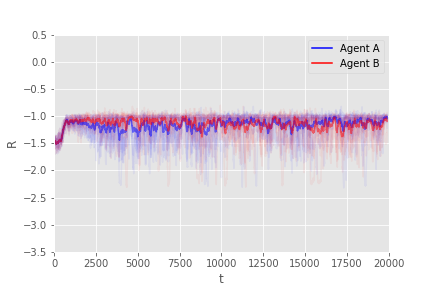
\includegraphics[height=1.8in]{figures/QvsQ}}%
  \subfigure[FP$Q$-learner (blue) vs $Q$-learner (red)]{%
  \label{fig:FPQvsQ}%
  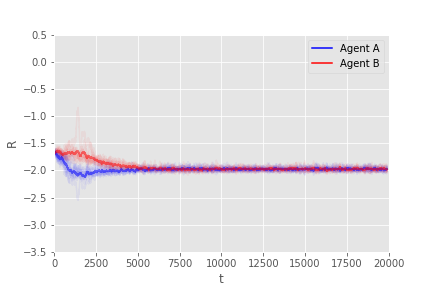
\includegraphics[height=1.8in]{figures/FPQvsQ}}%
  \caption{Rewards obtained in IPD. We plot the trajectories of 10 simulations with shaded colors. Darker curves depict mean rewards. }\label{fig:IPD}
  
 \subfigure[$Q$-learner vs $Q$-learner]{%
\label{fig:QvsQ_SH}%
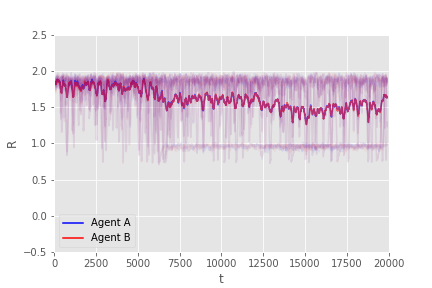
\includegraphics[height=1.8in]{figures/QvsQ_SH}}%
\subfigure[FP$Q$-learner (blue) vs $Q$-learner (red)]{%
\label{fig:FPQvsQ_SH}%
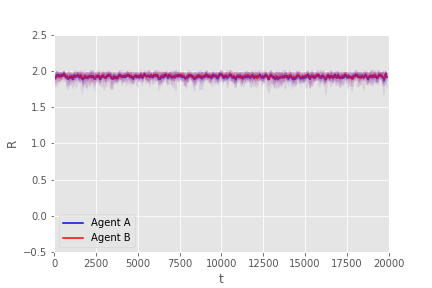
\includegraphics[height=1.8in]{figures/FPQvsQ_SH}}%
\caption{Rewards in ISH game}\label{fig:ISH}

\subfigure[$Q$-learner vs $Q$-learner]{%
\label{fig:QvsQ_C}%
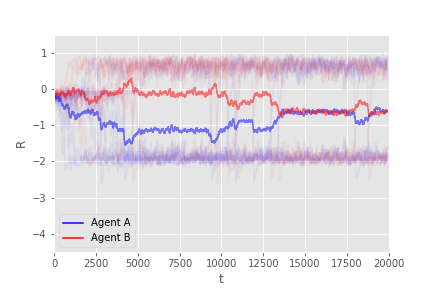
\includegraphics[height=1.8in]{figures/QvsQ_C}}%
\subfigure[FP$Q$-learner (blue) vs $Q$-learner (red)]{%
\label{fig:FPQvsQ_C}%
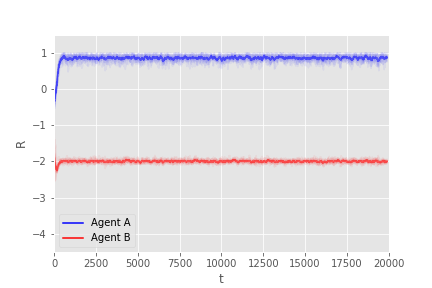
\includegraphics[height=1.8in]{figures/FPQvsQ_C}}%
\caption{Rewards in IC game}\label{fig:IC}

\end{figure*}

We turn to another social dilemma game, the Stag Hunt game, in which both agents must coordinate 
to maximize their rewards. They payoff matrix is in Table \ref{tab:payoffSG}, with
two Nash equilibria (C,C) and (D,D). We designate its iterated version ISH. We use the same experimental setting as before and report results in Figure \ref{fig:ISH}. 

\begin{table}[h!]
\begin{center}
\begin{tabular}{c|c|c}
\hline
 & C & D \\
\hline
C & (2, 2) & (0, 1) \\
\hline
D & (1, 0) & (1, 1)  \\
\hline
\end{tabular}
\end{center}
\caption{Payoff Matrix of Stag Hunt}
\label{tab:payoffSG}
\vspace{-2ex}
\end{table}
\noindent Once again, the independent learning solution cannot
cope with the non-stationarity of the environment and oscillates between both
equilibria  without clear convergence to one of 
them (Fig. \ref{fig:QvsQ_SH}). On the other hand, the FP$Q$-learner converges quite rapidly to the socially optimal policy (Fig. \ref{fig:FPQvsQ_SH}). Then, the environment becomes
essentially stationary to its opponent, who also converges to that policy.


% \begin{figure*}[h!]
% \centering
% \subfigure[$Q$-learner vs $Q$-learner]{%
% \label{fig:QvsQ_SH}%
% 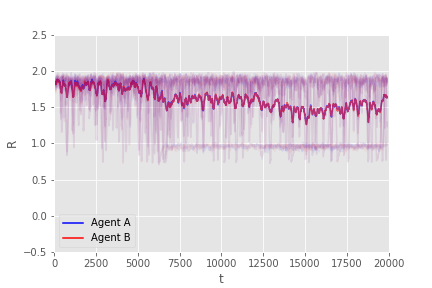
\includegraphics[height=1.8in]{figures/QvsQ_SH}}%
% \subfigure[FP$Q$-learner (blue) vs $Q$-learner (red)]{%
% \label{fig:FPQvsQ_SH}%
% 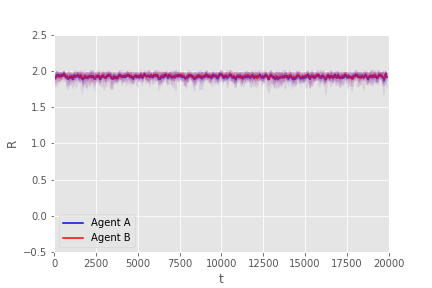
\includegraphics[height=1.8in]{figures/FPQvsQ_SH}}%
% \caption{Rewards obtained in the iterated stag hunt game}\label{fig:ISH}
% \end{figure*}

The last social dilemma that we consider is the Chicken game, with payoff matrix in Table \ref{tab:payoffC}. It has two pure Nash equilibria (C, D) and (D,C). We designate its iterated variant by IC.

\begin{table}[h!]
\begin{center}
\begin{tabular}{c|c|c}
\hline
 & C & D \\
\hline
C & (0, 0) & (-2, 1) \\
\hline
D & (1, -2) & (-4, -4)  \\
\hline
\end{tabular}
\end{center}
\caption{Payoff Matrix of Chicken}
\label{tab:payoffC}
\vspace{-2ex}
\end{table}
% \begin{figure*}[h!]
% \centering
% \subfigure[$Q$-learner vs $Q$-learner]{%
% \label{fig:QvsQ_C}%
% 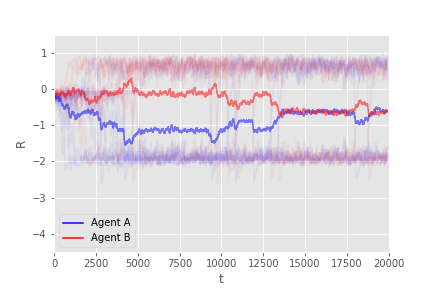
\includegraphics[height=1.8in]{figures/QvsQ_C}}%
% \subfigure[FP$Q$-learner (blue) vs $Q$-learner (red)]{%
% \label{fig:FPQvsQ_C}%
% 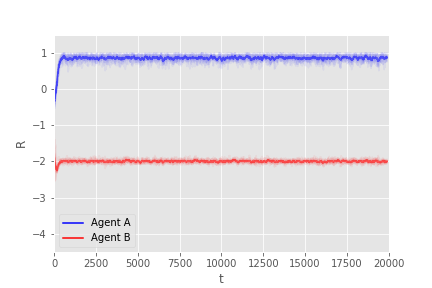
\includegraphics[height=1.8in]{figures/FPQvsQ_C}}%
% \caption{Rewards obtained in the iterated chicken game}\label{fig:IC}
% \end{figure*}
\noindent 
Figure \ref{fig:QvsQ_C} depicts 
again the ill convergence due to lack of opponent awareness in the
independent $Q$-learning case; note that the instabilities continued cycling
even after the limit in the displayed graphics. Alternatively, the DM
with opponent modelling has an advantage and converges to her optimal Nash
equilibrium (D,C) (Fig. \ref{fig:FPQvsQ_C}).

\begin{figure*}[!ht]%
\centering
\subfigure[FP$Q$-learner (blue) vs WoLF-learner (red)]{%
  \label{fig:L1vsWoLF_C}%
  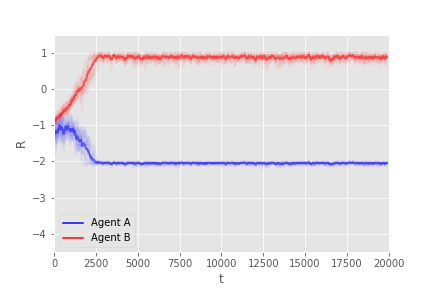
\includegraphics[height=1.8in]{figures/L1vsWoLF_C}}%
  \subfigure[L2$Q$-learner (blue) vs WoLF-learner (red)]{%
  \label{fig:L2vsWoLF_C}%
  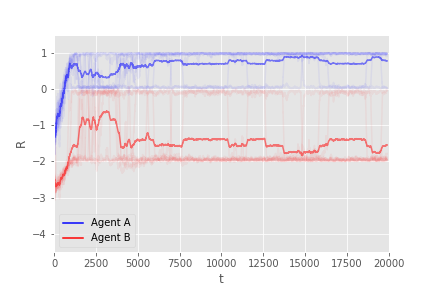
\includegraphics[height=1.8in]{figures/L2vsWoLF_C}}%
  \caption{Rewards obtained in the IC game against a WoLF-PHC adversary. }
\end{figure*}

{\color{black}
In addition, we study another kind of opponent to show how our framework
can adapt to it. We consider an adversary that learns according to the
WoLF-PHC algorithm \cite{bowling2001rational}, one of the best learning approaches in the multi-agent reinforcement learning literature. Figure \ref{fig:L1vsWoLF_C}
depicts a FP$Q$-learner (level-$1$) against this adversary, where the latter 
clearly exploits the former. However, if we go up in the level-$k$ hierarchy and model our
DM as a level-$2$ $Q$-learner, she outperforms her
opponent (Fig. \ref{fig:L2vsWoLF_C}).}



%%%%%%%%%%%%%%%%%%%%%%%%%%%%%%%%%%%%%%%%%%%%%%%%%%%%%
\subsubsection{Repeated Matrix Games With Memory}\label{sec:mem}

Section \ref{kk2} illustrated the ability of the modelled agents
to effectively learn Nash equilibrium strategies in several iterated games.
However, if we let agents have memory of previous movements, other types
of equilibria may emerge, including those in which agents cooperate. We can easily augment the agents to have memory of the past $T$ joint actions taken. However, \cite{press2012iterated} proved that, in the IPD, agents with a good memory-1 strategy can effectively force the iterated game to be played as memory-1, ignoring longer play histories. Thus, we resort to memory-1 iterated games.

We restrict our attention to the IPD. We model the memory-1 IPD as a TMDP in which the state $\mathcal{S}$ adopts the form $s_t = (a_{t-1}, b_{t-1}), \,\,  t > 0$
describing the previous joint action, plus the initial state $s_0$ in which there
is no prior action. Note that now the DM's policy is conditioned on
$\mathcal{S}$, and it is fully specified by the probabilities
$\pi(C | CC)$, $\pi(C | CD)$, $\pi(C | DC)$, $\pi(C | DD)$, and  $\pi(C | s_0)$.

\begin{figure}[h!]
\centering
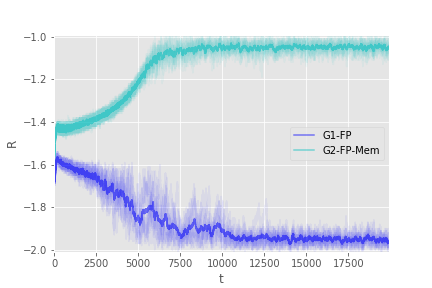
\includegraphics[scale=0.5]{figures/MemvsTFT_G1}%
\caption{Rewards obtained by the DM for players: FPQ memoryless player vs TFT player (G1) and FPQ memory-1 player vs TFT player (G2).}\label{fig:Mem1}
\end{figure}

\noindent We assume a stationary adversary playing Tit-For-Tat (TFT), i.e.\ replicating
the opponent's previous action \cite{axelrod84}. TFT is a Nash equilibrium in the IPD with memory.
We aim at showing that the supported DM is able to learn the equilibrium strategy. 

In the experiments, the adversary will compete with either an agent playing FP (the same from the stateless environment), or with a memory-1 agent also playing FP. Figure \ref{fig:Mem1} represents the utilities attained by these agents in both duels. As can be seen, a memoryless FPQ player cannot learn an optimal policy and forces the TFT agent to play defect. In contrast, augmenting this agent to have memory of the previous move allows him to learn the optimal policy (TFT), that is, he learns to cooperate, leading to a higher cumulative reward.

\subsubsection{Discussion}

We have shown through our examples some qualitative properties of the proposed framework. Explicitly modelling an opponent (as in the level-1 or FP$Q$-learner) is beneficial to maximize the rewards attained by the DM, as shown in the ISH and IC games. In both games, the DM obtains higher reward as a level-1 thinker than as a naive $Q$-learner against the same opponent. Also, going up in the hierarchy helps the DM to cope with more powerful opponents such as the WoLF-PHC algorithm.

In the two previous games, a level-1 DM makes both her and her opponent reach a Nash equilibrium, in contrast with the case in which the DM is a naive learner, where clear convergence is not assured. In both games there exist 
two pure Nash equilibria, and the higher-level DM achieved the most profitable one for her, effectively exploiting her adversary.

The case of the IPD is specially interesting. Though the level-1 DM also converges to the unique Nash equilibrium (Fig. \ref{fig:FPQvsQ}), it obtains less reward than its  naive counterpart (Fig. \ref{fig:QvsQ}). Recall that the naive $Q$-learner 
would remain exploitable by another opponent. We argue that the FP$Q$-learner did not learn to cooperate, and thus achieves lower rewards, due to the specification of the game and not as a limitation of our approach. To allow for the emergence of cooperation in the IPD, agents should remember past actions taken by all players. If we specify an environment in which agents recall the last pair of actions taken, the FP$Q$-learner is able to cooperate (Fig. \ref{fig:Mem1}) with an opponent that plays a Nash optimum strategy in this modified setting, Tit-For-Tat. 
\fi
% We believe that a high level $k$ (i.e., fictitious play versus opponent-unawareness) should be needed in order to internalize an adversary playing TFT.

% \subsubsection{Potential experiments}

% Maybe test also on some coordination games, such as the repeated variant of Stag Hunt \cite{skyrms2004stag}?

% Then, we may compute some social metrics (such as social utility $\frac{R_1 + R_2}{2}$) as introduced by \cite{perolat2017multi} and see if scores are better with a high k-level instead of with just independent $Q$-learning. 

% (i.e., to be a good social individual you have to model opponents)


%%%%%%%%%%%%%%%%%%%%%%%%%%%%%%%%%%%%%%%%%%%%%%%%%%
%\subsection{AI Safety Gridworlds and Markov Security Games against misspecified %adversary}\label{s:sg}
%\subsection{AI SAFETY GRIDWORLDS}
\subsection{Advantages of modelling adversaries}\label{s:sg}

We demonstrate first that  by
explicitly modelling the behaviour of adversaries, 
our framework improves upon $Q$-learning methods. 
%yielding higher rewards to the DM.
For this, we consider a suite of recent RL safety benchmarks
 introduced in \cite{leike2017ai}.
Our focus is 
on the safety \emph{friend or foe} environment:
the supported DM
needs to travel through a room and choose 
between two identical boxes, respectively hiding a positive
and a negative reward (+50 and -50, respectively), controlled by
an adaptive opponent.
This may be interpreted as a spatial Stackelberg game in which
the adversary is planning to attack one of two targets; the defender
will obtain a positive reward if she travels to the chosen target. Otherwise,
she will miss the attacker and incur in a loss.

As \cite{leike2017ai} shows, a \emph{deep $Q$-network}
(and, similarly, the independent tabular $Q$-learner as we show) fails to
achieve optimal results since the reward process is controlled by the adversary.
%\textcolor{red}{An alternative approach to security games in spatial domains was introduced in \cite{klimamarkov}. The authors extend the single-agent $Q$-learning algorithm with an adversarial policy selection inspired by the EXP3 rule from the \emph{adversarial multi-armed bandit} %(AMAB) framework in \cite{auer1995gambling}.  However, their approach does not explicitly model an adversary.}

Figure \ref{fig:friendorfoe} shows the initial set up. 
Cells 1 and 2 depict the adversary's targets, who decides which 
one will 
hide the positive reward.

\begin{figure}
   \centering
   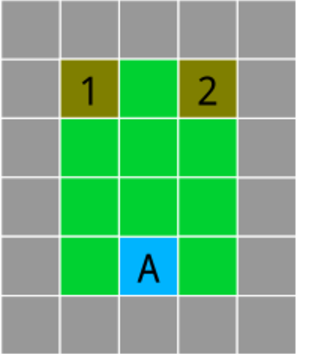
\includegraphics[scale=0.5]{figures/friend-or-foeCUT}
    %\fbox{\rule[-.5cm]{0cm}{4cm} \rule[-.5cm]{4cm}{0cm}}
   \caption{\emph{Friend or foe} environment from the AI Safety Gridworlds benchmark \cite{leike2017ai}.
   The blue cell 
represents the DM's initial state, gray cells represent the walls of the room.   } \label{fig:friendorfoe}
 \end{figure}


%%%%%%%%%%%%%%%%%%%%%%%%%%%%%%%%%%%%%%%%%
\subsubsection{Stateless Variant}\label{sec:statv}

Consider a simplified initial setting with a single state and
two actions. As in  \cite{leike2017ai}, the adaptive
opponent estimates the DM's actions using an exponential smoother.
Let $\bm{p} = (p_1, p_2)$ be the probabilities
with which the DM will, respectively, choose targets 1 or 2
as estimated by the adversary. 
Initial estimates %of the target preferred by the DM 
are
$\bm{p} = (0.5, 0.5)$.
After each iteration, the update is %t every iteration, he updates his knowledge
%through 
$
\bm{p} := \beta \bm{p} + (1 - \beta ) \bm{a},
$
with $0 < \beta < 1$ 
a learning rate, unknown from the DM's point of view,
and $\bm{a} \in \lbrace (1, 0), (0, 1) \rbrace$ is a one-hot encoded
vector respectively indicating whether the DM  chose targets 1 or 2. 
Assume an adversary which places the positive reward in target
$t = \argmin_i (\bm{p})_i$.
%Then, we consider three different environments, depending on the type of adversary:
% \begin{itemize}
% \item \emph{Friendly opponent.} Places the positive reward in target $t = \argmax_i (\bm{p})_i$.
% \item \emph{Adversarial opponent.} Places the positive reward in target $t = \argmin_i (\bm{p})_i$.
% \item \emph{Neutral opponent.} Places the positive reward in target 1 with constant probability $p$.
% \end{itemize}
%As an example, at the beginning of a game, the opponent has estimates $\bm{p} = (0.5, 0.5)$ of the preferred target for the DM. 
 %If she chooses target 1, then the opponent's estimate of $p_1$ will increase. Henceforth, in the next round he will place the positive reward in target 2, and so on.


%{\color{blue} ver qué se hace finalmente con lo de dirichlet con olvido}
Since the DM has to deal with a strategic adversary, 
consider a variant of FP$Q$-learning (section 3.1) giving
more relevance to more recent actions.
Algorithm \ref{alg:duwff} provides a modified update 
scheme, based on the the property that the Dirichlet distribution is conjugate of the Categorical distribution: 
 instead of weighting all observations equally,
 we essentially account for just the last $\frac{1}{1 - \lambda}$ 
 opponent actions.  
 \begin{algorithm}
\begin{algorithmic}
\State Initialize pseudocounts $ \bm{\alpha^0} = (\alpha^0_1, \ldots, \alpha^0_n)$
\For{$t = 1, \ldots, T $}
\State $\bm{\alpha^t} = \lambda \bm{\alpha^{t-1}}$ \Comment Reweight with factor $0 < \lambda < 1$
\State Observe opponent action $b^t_i, i \in \lbrace b_1, \ldots, b_n \rbrace$
\State $\alpha^t_i = \alpha^{t-1}_i + 1$ \Comment Update posterior
\State $\alpha^t_{-i} = \alpha^{t-1}_{-i}$
\EndFor
\end{algorithmic}
\caption{Dirichlet updating with forget factor}
\label{alg:duwff}
\end{algorithm}

For a level-2 defender, as we do not know 
the actual rewards of the adversary (modelled as a level-1 learner), 
 we  model it as in a zero-sum scenario  ($r_B = -r_A$) making this case similar to the Matching Pennies game. The adopted discount factor is $\gamma = 0.8$;
 there are $5000$ episodes; the initial exploration parameter
 is $\epsilon = 0.1$ and the learning rate, $\alpha = 0.1$. The 
 assumed 
 forget factor is $\lambda = 0.8$.
\begin{figure}%
\centering
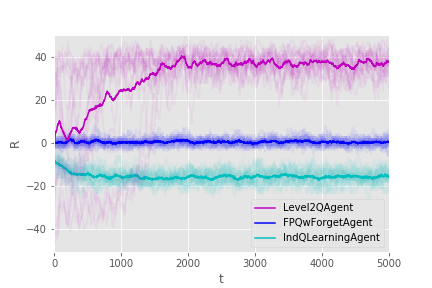
\includegraphics[scale=0.5]{figures/4C_08_adversary}%
\caption{Rewards for the DM against the adversarial opponent}\label{fig:4C_adv}
\end{figure}
 Figure \ref{fig:4C_adv} displays results. We consider three defenders:
an opponent unaware $Q$-learner; a level-1 DM with forget
using Algorithm \ref{alg:duwff}; and a
level-2 agent. The first defender is clearly is exploited by the adversary 
achieving suboptimal results (rewards close to -20).
In contrast, the level-1 DM with forget effectively
learns a stationary optimal policy (reward 0). Finally, the
level-2 agent is capable of exploiting 
the adaptive adversary actually achieving positive rewards
(around 40, close to the upper bound of 50 due to the value of the positive reward). 

%Even though the adversary is not exactly a level-1 $Q$-learner, making the DM a level-2 agent gives sufficient advantage.
Note that the actual adversary behaves differently from how the DM models him,
as he is not a level-1 $Q$-learner. Even so, modelling him as 
such, gives the DM sufficient advantage in this case.
This robustness against opponent misspecification emerges as an
advantage of our proposed framework.

We next perform a similar experiment replacing the $\epsilon-$greedy
policy with a softmax one: actions at state $s$ are taken with probabilities 
proportional to $Q(s, a)$. Figure \ref{fig:softmax}
provides several simulation runs of a level-2 $Q$-learner versus the adversary,
showing that, indeed, changing the policy sampling scheme does not worsen
the DM with respect to the $\epsilon-$greedy alternative.

\begin{figure}[h!]
\centering
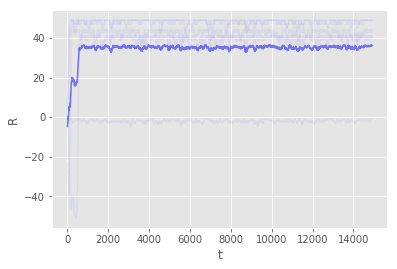
\includegraphics[scale=0.5]{figures/softmax.png}%
\caption{Rewards for the DM against the adversarial opponent, using a softmax policy.}\label{fig:softmax}
\end{figure}

Lastly, we tried other models for the opponent's rewards $r_B$. Instead of observing the opponent reward as $r_B = -r_A$ in a zero-sum setting, where $r_B \in \lbrace -50, 50 \rbrace$,  we tried two additional reward scalings $r_B \in \lbrace -1, 1 \rbrace$ and $r_B \in \lbrace 0, 1 \rbrace $. Figure \ref{fig:4C_rs} displays the result, portraying
similar results qualitatively.
%Maybe it will be significant with a DQN, as reported in \url{https://arxiv.org/pdf/1709.06560.pdf}.

 \begin{figure}%
 \centering
 \subfigure[Rewards $+1$ and $0$ for the adversary]{%
 \label{fig:4C_binary_adv}%
 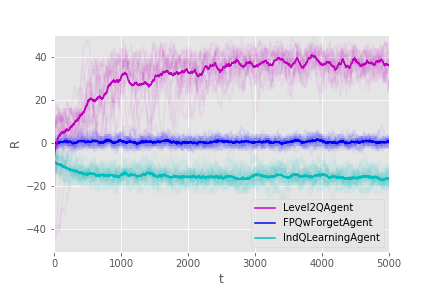
\includegraphics[scale=0.5]{figures/4C_08_binaryadversary}}%
 \subfigure[Rewards $+1$ and $-1$ for the adversary]{%
 \label{fig:4C_binary_1m1}%
 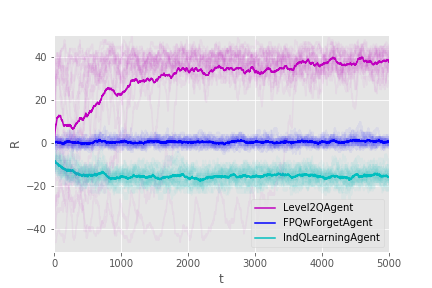
\includegraphics[scale=0.5]{figures/4C_08_1m1adversary}}%
 \caption{Rewards against same adversary (exp. smoother) using different reward scalings.}\label{fig:4C_rs}
 \end{figure}

%%%%%%%%%%%%%%%%%%%%%%%%%%%%%%%%%%%%%%%%%%%%%%%%%
\subsubsection{Facing more powerful adversaries}

So far, the DM has interacted against an exponential smoother
adversary. This may be exploited if the DM is a level-2 agent.
%according to the proposed hierarchy.
We study now the outcome of the process
when we consider more powerful adversaries.

First, we parameterize our opponent as a level-2 $Q$-learner.
To do so, we specify the rewards he receives as $r_B = -r_A$
(for simplicity we consider a zero-sum game, although our framework allows dealing with the general-sum case). Figure \ref{fig:L2vsL2} depicts the rewards for both the DM (blue)
and her adversary (red). We have computed the frequency of choosing each of the actions, and both players select either action 
with probability $0.5 \pm 0.002$ based on 10 different random seeds. Both agents achieve the Nash equilibrium, consisting of
choosing between both
actions with equal probability, leading to an expected cumulative reward of 0, as shown in the graph.

\begin{figure*}%
\centering
\subfigure[L2$Q$-learner (blue) vs L2$Q$-learner (red)]{%
  \label{fig:L2vsL2}%
  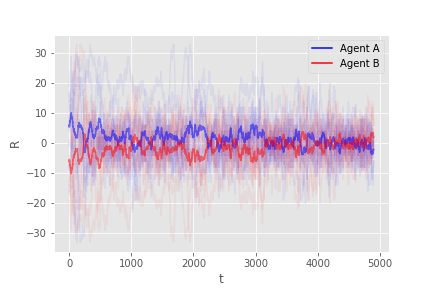
\includegraphics[height=1.4in]{figures/L2Q_vs_L2Q.png}}%
  \subfigure[L3$Q$-learner (blue) vs L2$Q$-learner (red)]{%
  \label{fig:L3vsL2}%
  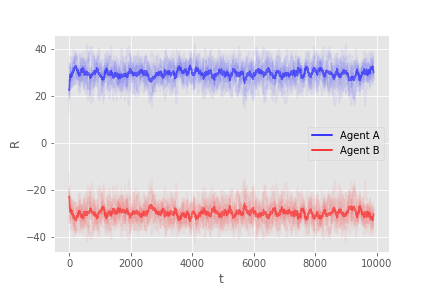
\includegraphics[height=1.4in]{figures/L3Q_vs_L2Q.png}}%
  
  \subfigure[L3$Q$-learner (blue) vs L1$Q$-learner (red)]{%
  \label{fig:L3vsL1}%
  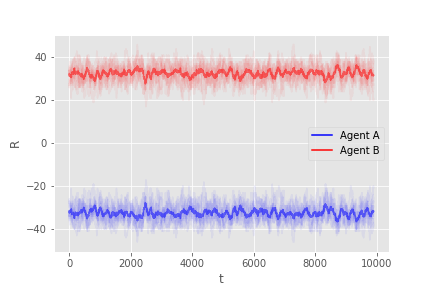
\includegraphics[height=1.4in]{figures/L3_vs_L1.png}}%
  \subfigure[L3$Q$-learner with opponent averaging (blue) vs L1$Q$-learner (red)]{%
  \label{fig:L3DirvsL1}%
  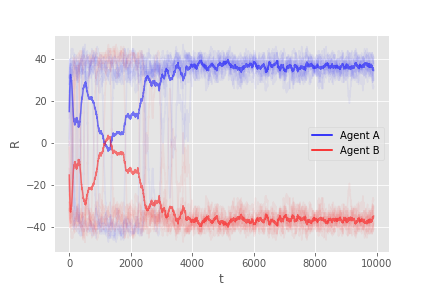
\includegraphics[height=1.4in]{figures/L3Dir_vs_L1.png}}%
  
  \subfigure[Estimate of  $P_{L1Q}$: DM's belief that her opponent is a level-1 $Q$-learner]{%
  \label{fig:probas}%
  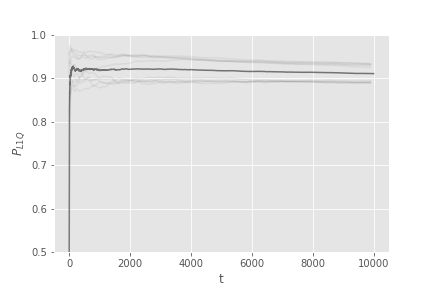
\includegraphics[height=1.4in]{figures/probs.png}}%  

  
  \caption{Rewards obtained against the exponential smoother adversary. }
\end{figure*}

Increasing the level of our DM to make her level-3, allows her to exploit a level-2 adversary, Fig. \ref{fig:L3vsL2}. However, this DM fails to exploit a level-1 opponent, i.e., a FP$Q$-learner, Fig. \ref{fig:L3vsL1}. The explanation to this apparent paradox is that the DM is modelling her opponent as a more powerful agent
than he actually is: her model is inaccurate and leads to poor performance.
However, this ``failure" suggests a potential solution to the problem
using type-based reasoning (Section \ref{sec:com}). Figure \ref{fig:L3DirvsL1} depicts the rewards of a DM that keeps track of both level-1 and level-2 opponent models and learns, in a Bayesian manner, which one is she 
actually facing. The DM keeps estimates of the probabilities $P_{L1Q}$ and $P_{L2Q}$ that her opponent is acting as if he was a level-1 or a level-2 $Q$-learner, respectively. Figure \ref{fig:probas} depicts the evolution of $P_{L1Q}$: we observe that it places most of the probability in the correct opponent type. 


%Maybe from the safety part cite something from \cite{maliciousAIreport} and/or \cite{amodei2016concrete}?

% \subsection{Markov Security Games}

% An extension of Stackelberg or security games to spatial domains was introduced in \cite{klimamarkov}. They extend the single-agent $Q$-learning algorithm with an adversarial policy selection inspired by the EXP3 rule from the \emph{adversarial multi-armed bandits} (AMAB) framework \cite{auer1995gambling}. Though robust, their approach does not explicitly model an adversary, nor is amenable to function approximation of the $Q$-function, thus scaling poorly as the number of states increases.

% We test ...



%\subsection{Pong's Dilemma?}

%Or some other 2-player game..

%\subsection{3D control tasks}

%We could apply to some robot locomotion tasks under adversaries, such as the settings introduced in \cite{bansal2017emergent}.

%%%%%%%%%%%%%%%%%%%%%%%%%%%%%%%%%%%%%%%%%%
\subsubsection{Spatial Variant}


We now compare the independent $Q$-learner and a level-$2$ $Q$-learner against the
same adaptive exponential smoother opponent in the spatial gridworld domain
in Fig. \ref{fig:friendorfoe}. The DM has four actions to choose, one for each direction in which the DM is allowed to move for one step. Target rewards 
are delayed until the DM arrives at one of the pertinent locations, 
obtaining $\pm 50$ depending on the target chosen by the adversary.
Each step is penalized with -1 for the DM. Episodes end at a maximum of 50 steps or when the agent arrives first at targets 1 or 2. 
The discount factor is $\gamma = 0.8$ and $15000$ episodes are 
considered. For the level-2 agent, we consider different exploration hyperparameters, $\epsilon_A$ and $\epsilon_B$ for the DM's policy and her correponding model for her opponent;
initially,  $\epsilon_A = \epsilon_B = 0.99$ with decaying rules $\epsilon_A := 0.995\epsilon_A$ and $\epsilon_B := 0.9\epsilon_B$ every $10$ episodes and learning rates $\alpha_2 = \alpha_1 = 0.05$. For the independent $Q$-learner, we set similar initial hyperparameters.

Results are displayed
in Figure \ref{fig:4C_gridworld}. Again, an independent $Q$-learner is
exploited by the adversary, obtaining even more negative results  
than in 
Figure \ref{fig:4C_adv} due to the penalty at each step. In contrast,
a level-2 agent approximately estimates adversarial
behavior, modelling him as a level-1 agent, obtaining positive rewards. Figure \ref{fig:L3Dir_spatial} depicts the rewards of a DM that maintains 
opponent models for both level-1 and level-2 $Q$-learners. Although the adversary is of neither class, the DM achieves positive rewards,
suggesting that the framework is capable of generalizing between opponent behaviours not exactly reflected by the DM's opponent model.
This shows that our level-$k$ thinking scheme it is sufficiently robust to opponent misspecification.

\begin{figure*}[h]
\centering
\subfigure[Rewards for various DM models]{%
  \label{fig:4C_gridworld}%
  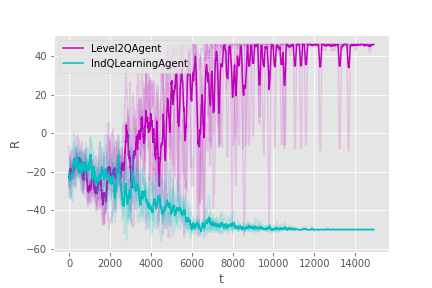
\includegraphics[scale=0.5]{figures/AI_safety}}%
  \subfigure[Rewards for a DM with opponent models for a L1 $Q$-learner and a L2 $Q$-learner (red)]{%
  \label{fig:L3Dir_spatial}%
  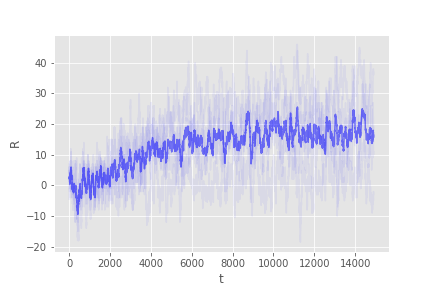
\includegraphics[scale=0.5]{figures/Level3Dir_vs_ExpSmoother.png}}%
  \caption{Rewards against the exponential smoother opponent in the spatial environment. }
\end{figure*}


Lastly, we also perform several experiments in which we try different values of the hyperparameters,  to further highlight the robustness of the framework. Table \ref{tab:rob} displays mean rewards (and standard deviations) for five different random seeds, over different hyperparameters of Algorithm \ref{alg:l2ur}. Except in the case where the initial exploration rate $\epsilon_0$ is set to a high value (0.5, which makes the DM achieve a positive mean reward), the other settings showcase that the framework (for the level-2 case) is robust to different learning rates.

\begingroup
\renewcommand{\arraystretch}{0.7}
\begin{table}[h]
\small
\caption{Hyperparameter robustness of Algorithm \ref{alg:l2ur} on the spatial gridworld.}\label{tab:rob}
\centering
\begin{tabular}{lllr}
\hline
$\alpha_2$ &  $\alpha_1$ & $\epsilon_0$ & Mean Reward \\
\hline
0.01 & 0.005 & 0.5 & $15.46 \pm 47.21$  \\
0.01 & 0.005 & 0.1 & $40.77 \pm 27.48$  \\
0.01 & 0.005 & 0.01 & $46.32 \pm 16.15$  \\\hline
0.01 & 0.02 & 0.5 & $15.58 \pm 47.17$  \\
0.01 & 0.02 & 0.1 & $43.05 \pm 23.65$  \\
0.01 & 0.02 & 0.01 & $47.81 \pm 10.83$  \\\hline
0.1 & 0.05 & 0.5 & $15.30 \pm 47.27$  \\
0.1 & 0.05 & 0.1 & $42.82 \pm 24.08$  \\
0.1 & 0.05 & 0.01 & $48.34 \pm 8.10$  \\\hline
0.1 & 0.2 & 0.5 & $15.97 \pm 47.03$  \\
0.1 & 0.2 & 0.1 & $43.05 \pm 23.66$  \\
0.1 & 0.2 & 0.01 & $48.51 \pm 6.96$  \\\hline
 0.5 & 0.25 & 0.5 & $15.95 \pm 47.04$  \\
 0.5 & 0.25 & 0.1 & $43.06 \pm 23.64$  \\
 0.5 & 0.25 & 0.01 & $48.41 \pm 7.68$  \\\hline
 0.5 & 1.0 & 0.5 & $15.19 \pm 47.31$  \\
 0.5 & 1.0 & 0.1 & $42.98 \pm 23.71$    \\
 0.5 & 1.0 & 0.01 & $48.53 \pm 6.82$  \\\hline
\end{tabular}
\end{table} 
\endgroup
%%%%%%%%%%%%%%%%%%%%%%%%%%%%%%%%%%%%%%%%%%%%%%%%%%%%%%%
\subsection{Facing multiple opponents}

We illustrate the multiple opponent concepts from Section \ref{sec:mul} introducing a novel suite of  resource allocation experiments 
relevant in security settings. They are based on a modified version of Blotto games \cite{hart2008discrete}: the DM needs to distribute limited
resources over several positions susceptible of being attacked. Each of the attackers has to choose different positions
to deploy their attacks. Associated with each of the attacked positions there is a positive (resp. negative) reward with value 1 (-1). If the DM 
deploys more resources than the attackers in a particular position, she wins the positive reward and the negative one will be equally split  between
the attackers that chose to attack such position. If the DM deploys less resources, she will receive
the negative reward and the positive one will be equally split between the corresponding attackers.
In case of a draw, no player receives any reward.  

% We tested the several opponents extension of TMDPs presented in Section \ref{sec:mul} in this environment, restricting to the case of non-cooperative opponents. 

We compare the performance of a FP$Q$-learning agent vs a standard $Q$-learning agent, when facing two conditionally independent opponents both using 
exponential smoothing to estimate the probability of the DM placing a resource at each position, and implementing the attack where
this probability is the smallest (obviously both opponents perform exactly the same attacks).

Consider
a problem of defending three different positions; the DM needs to allocate two resources among such positions. For both the $Q$-learning and the FP$Q$-learning agents the discount factor will be $\gamma = 0.96$, $\epsilon = 0.1$ and the learning rate  $0.1$.%There are two non cooperative attackers and each of them must decide the position where his attack will be executed. 
%
As Fig. \ref{fig:2expsmoothers} shows, FP$Q$-learning is able to learn the opponents strategies and thus is less exploitable than standard $Q$-learning.
This experiment showcases the suitability of the framework to deal with multiple, independent adversaries, by straightforwardly extending the level-$k$ thinking scheme as discussed (Section \ref{sec:mul}).
\begin{figure}%
\centering
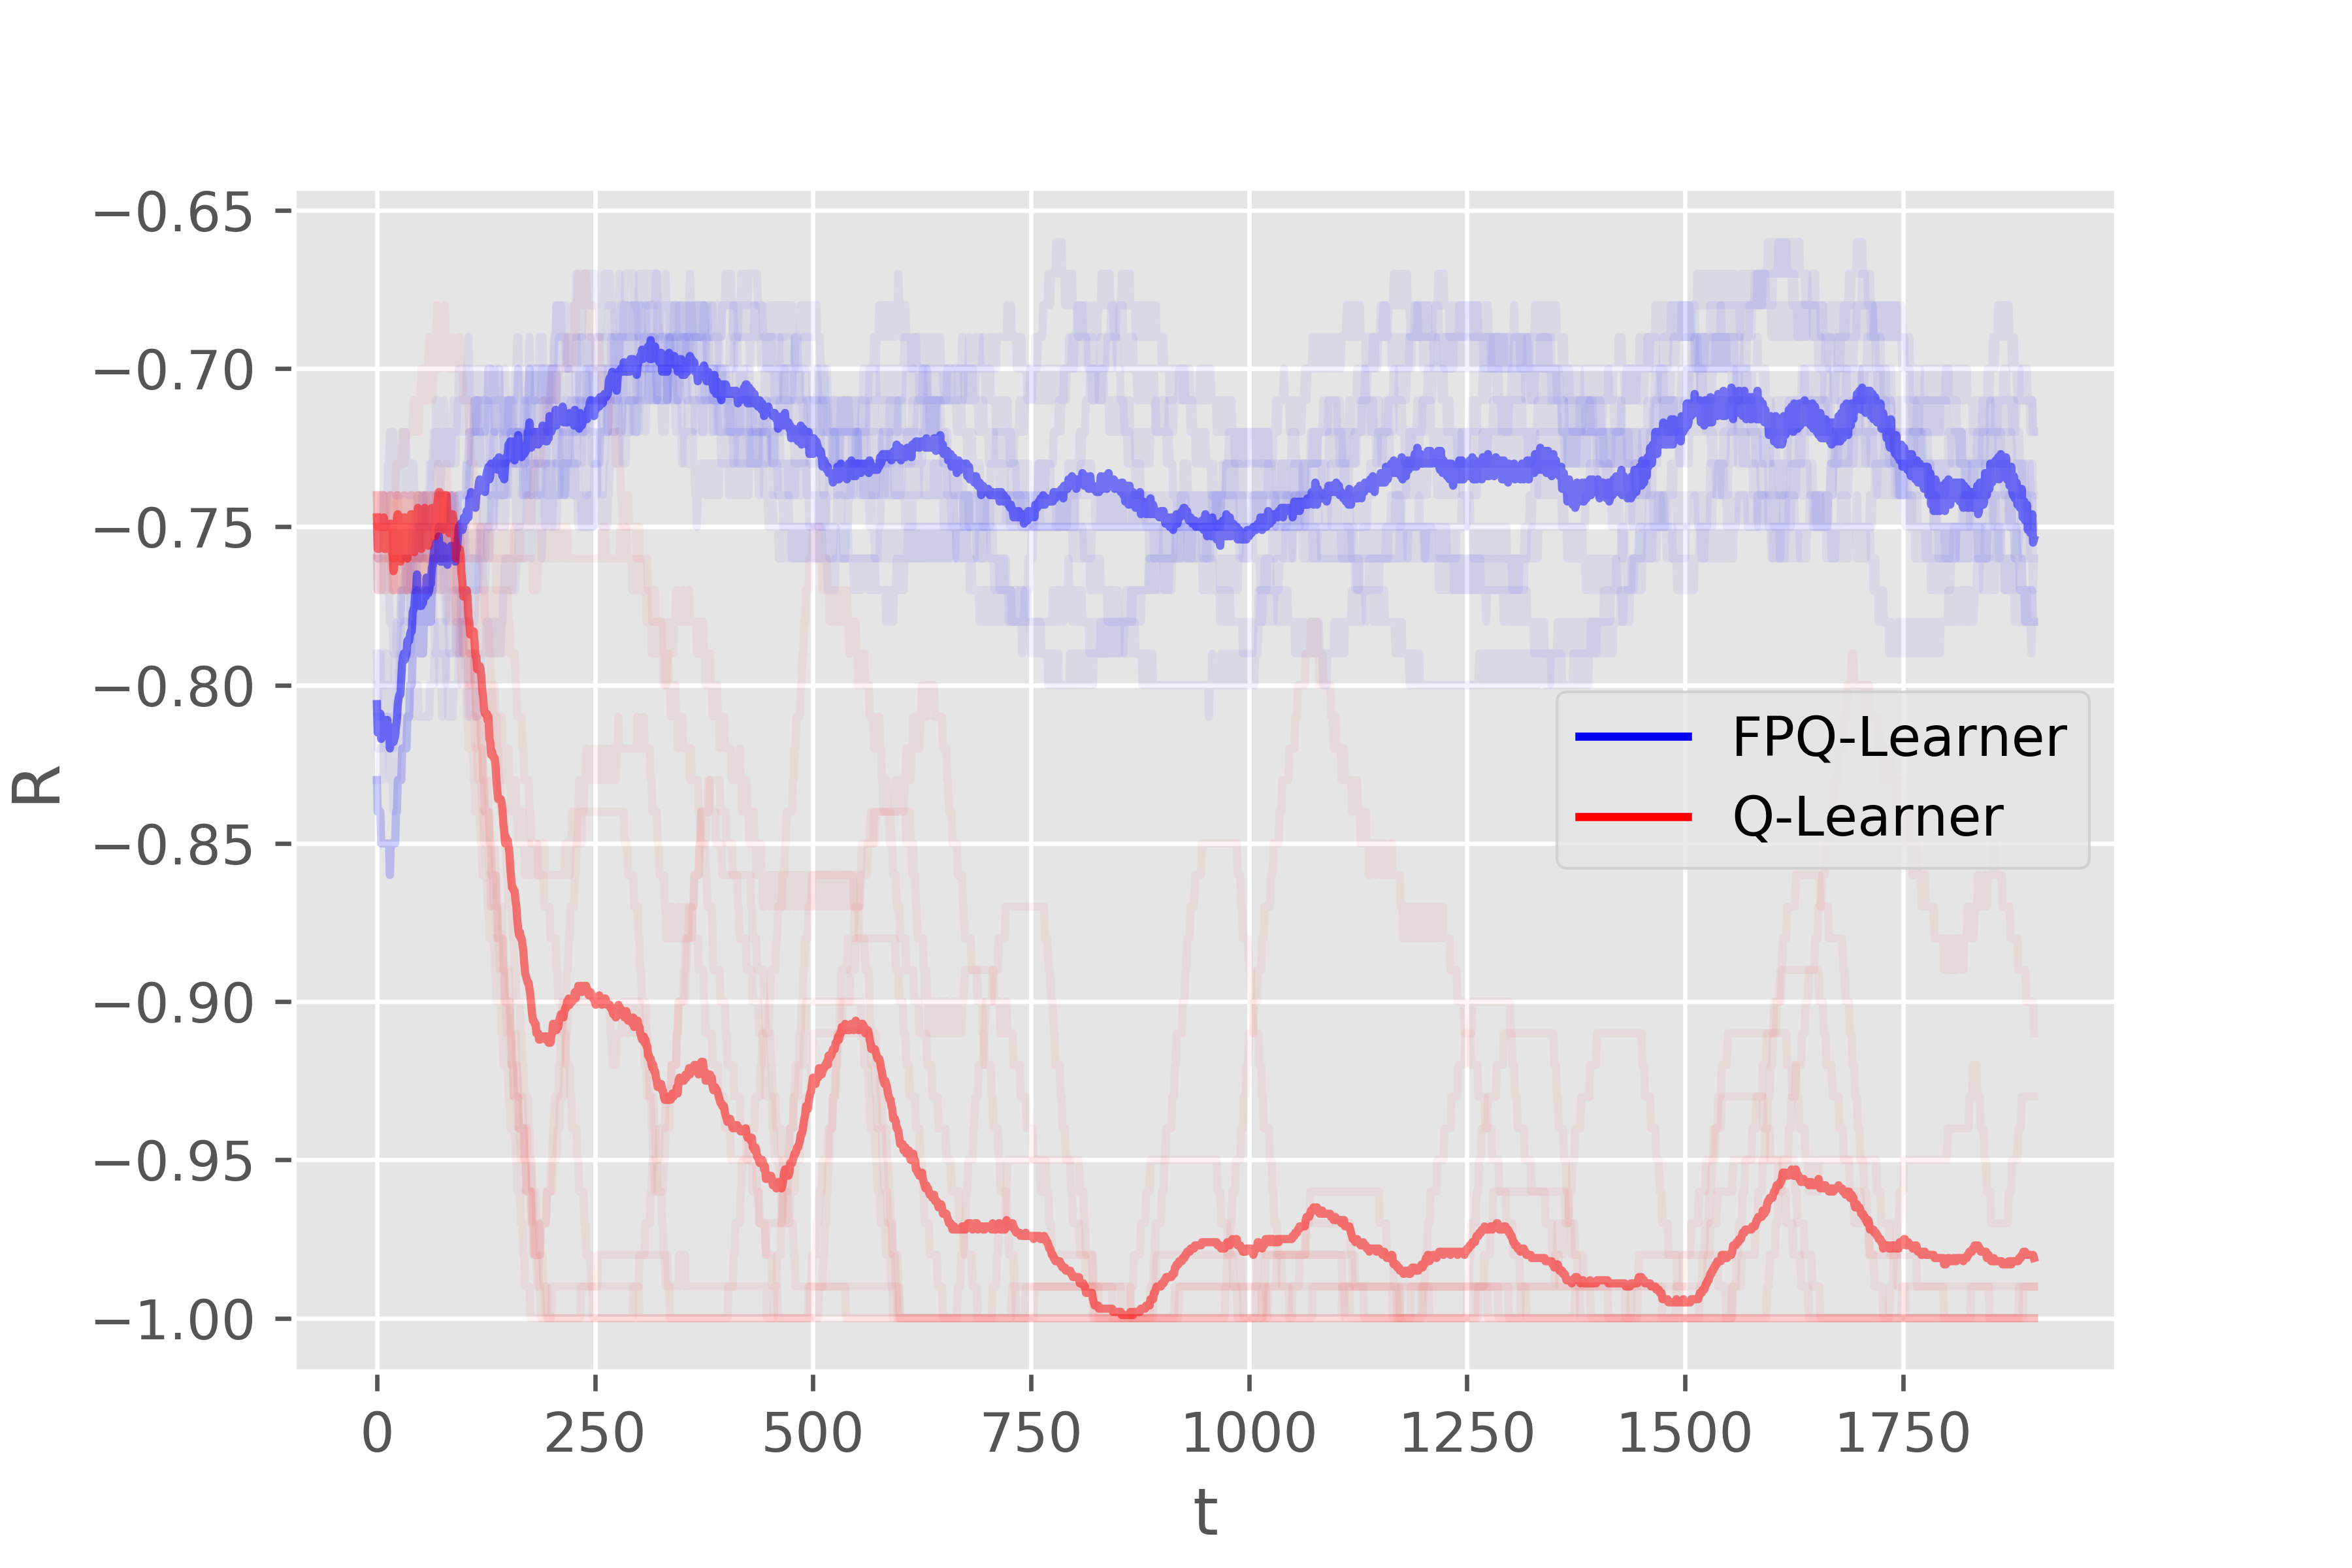
\includegraphics[scale=0.5]{figures/2expsmoothers.png}%
\caption{Rewards for the DM against the opponent}\label{fig:2expsmoothers}
\end{figure}
%



%In addition, we observe that depite the agent is assuming that the opponents he is facing are both stationary, which is not actually the case. %(Quizás quitar esto último...)

%More experiments:

%* Level-k? 
%* Two DIFFERENT exp smoothers.
%* ...


%\subsection{TMDPs for Urban Security Resource Allocation}

%We build upon the setting from \cite{ara_urban}. 

%\begin{itemize}
%    \item FPQ and $Q$ learner against a stationary opponent.
%    \item L2 and L1 against exponential smoother?.
%\end{itemize}

\subsection{Experiments with function approximation}\label{sec:cg}

We run a battery of experiments to showcase 
how our framework is actually compatible with variants in which $Q$-values are approximated with a parametric function, in particular a deep learning model, as in Section \ref{sec:approx}.

\begin{figure}[h]
\centering
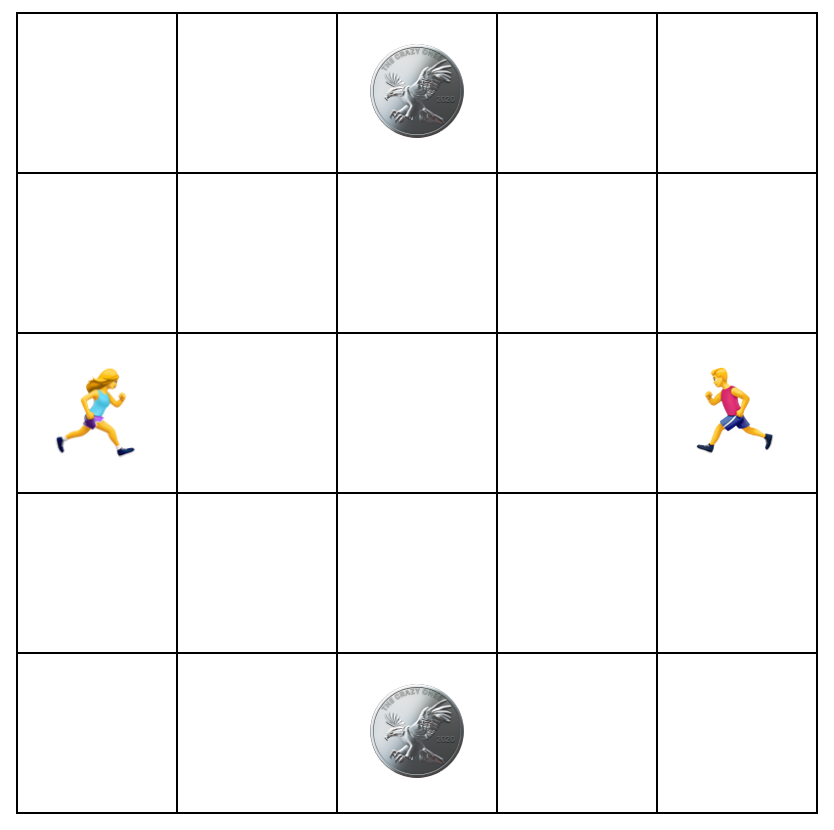
\includegraphics[scale=0.3]{figures/game5x5.png}%
\caption{An initial state for the Coin Game}\label{fig:coingame}
\end{figure}

For this, we create the gridworld game in Figure \ref{fig:coingame}. It is 
is played over an $N \times N$ grid ($N=5$ in the Figure). Each turn, both players (blue and red) move in either of the four directions (unless they try to cross the boundary of the grid), with the objective of chasing two different coins in the grid. For each coin the agent picks, he receives a reward of 1, unless the other agent arrives also at the same location,
in which case the perceived reward is only 0.5. 
Thus, this gridworld game can be cast as a coordination game.
The episode ends after 12 steps (so that each agent has ample time to pick both coins). 

The space of states is given as a $N \times N \times 4$ array, in which each of the four last slices denote the position of each player and coin as a one-hot encoded $N \times N$ matrix. A straightforward application of $Q$-learning would require a table $Q(s, a)$ with $(N \times N)^4 \times 4$ entries. Instead, we parameterize the $Q$-values to reduce the number of parameters: the state $s$ is flattened from a tensor in $\mathbb{R}
^{N \times N \times 4}$ to a vector in $\mathbb{R}
^{4N^2}$, and we project it to $\mathbb{R}^4$ using linear regression to obtain one $Q$-value for each of the four possible actions: 
given any state $s \in \mathbb{R}^{4N^2}$, we obtain the corresponding $Q$-value $Q(s, a)$ via $Q(s, a) = w_a^{\intercal}s $ with $w_a \in \mathbb{R}^{4N^2}$ being the weight vector for action $a$. Thus, we have reduced the total number of parameters to $N
^2\times 4 \times 4$. The extension to the $Q$-function approximator for the level-2 case is straightforward: instead of projecting to $\mathbb{R}^4$ we project to $\mathbb{R}^{4\times 4}$ to consider each pair of actions $(a, b)$, in order to approximate the corresponding $Q$-function $Q(s,a,b)$. 

Figures \ref{fig:coin1} and \ref{fig:coin2} depict the results of two games. In light color we depict the smoothed rewards along 10000 iterations for five different random seeds, and in darker colors the three averages of the $3 \times 5$ previous runs:
even in this approximate regime, a DM exhibiting higher rationality than its adversary can make an advantage from him. Thus, we have shown that our opponent modelling framework is compatible with approximate $Q$-values, being capable of harnessing all the benefits from the approximate regime, such as the reduced parameter count or generalization capabilities.
\begin{figure*}%
\centering
\subfigure[Rewards of two independent $Q$-learners against each other]{%
  \label{fig:coin1}%
  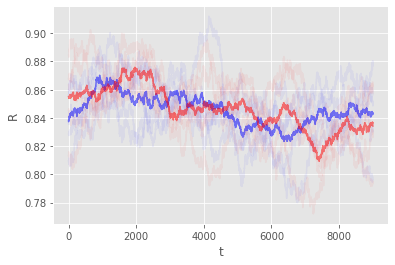
\includegraphics[scale=0.5]{figures/coin1}}%
  \subfigure[Rewards of a L2 $Q$-learner (blue) against an independent $Q$-learner (L0) (red)]{%
  \label{fig:coin2}%
  \hspace{0.2cm}
  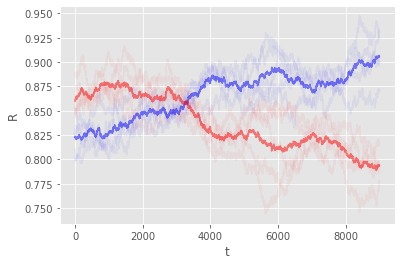
\includegraphics[scale=0.5]{figures/coin2.png}}%
  \caption{Rewards in the Coin Game using function approximators. }
\end{figure*}

Note we also used a multi-layer NN to parameterize the $Q$-functions, but we did not achieve a significant improvement in the results, so we just report those of the simplest model.


%%%%%%%%%%%%%%%%%%%%%%%%%%%%%%%%%%%%%%%%%%%%%%

\section{Data sharing: categories, agents and strategies}\label{sec:ds}
%In order to understand how to reach such solution, 
Next, we will move the second application introduced at the beginning of the chapter.
Before modeling interactions between data consumers and producers, it is convenient to understand the data categories available. 
Even though admittedly with a blurry frontier, 
from a legal standpoint, there are two main types:

\begin{itemize}
\item {\em Data that should not be bought/sold}. This refers to  
 personal information (PI), as e.g.\ the data preserved in the European
 Union through 
 the General 
 Data Protection Regulation (GDPR) \cite{gdpr} and other citizen defense frameworks
 aimed at guaranteeing civic liberties. PI includes 
 data categories such as 
%{\em  historical information}; 
{\em internal information} (like knowledge and beliefs, %authenticating, preferences, ethnicity, 
%sexual, %behavioral, demographics, 
%medical 
 and health %, and physical features
 data); 
{\em financial information} (like accounts or %; ownership; transactional;
 credit data);
{\em social information} (like %rofessional, 
criminal records %, public life, family, social network, and 
or communication data); or,
{\em tracking information} (like computer device; 
%contact method; 
or location data).
%
\item {\em Data that might be purchased}. Citizen’s data is a property,
there being a need to guarantee a fair and transparent compensation.
Accountability mitigates market frictions. For
traceability and transparency reasons,
blockchain-based platforms are being implemented at the moment within this domain.
\end{itemize}
%Of course, we acknowledge that the frontier between both
%categories %data that should not be sold and  that might be purchased 
  %is blurry.
  %Definitely,
  A characterization of what type of data 
  belongs to each category will depend on the context and is, most of the times, subjective.

In any case, in the last decades, modern data analytics techniques and strategies are enabling the generation of new types of data:
\begin{itemize}
\item {\em Data that might be estimated/derived.}  Currently available analytics technologies have the ability of estimating efficiently citizen behavior and other characteristics by deeply analyzing Big Data. For instance, platforms such as IBM Personality Insights \cite{ibm} estimate personality traits of a
given individual using his/her tweets, thus facilitating marketing activities.
As a result, the originating data becomes a new asset for a company
willing to undertake its analysis.
% If treated as a target, it derives in a new data asset of the company analyzing those data. 
\end{itemize}

Having mapped the available data, there is a need to understand the 
knowledge actually available and how is it uncovered.	
Within the above scenario, 
we consider two players in  a data 
sharing game: the data providers 
(Citizen, she) and the Dominant Data Owner (DDO, he).
A DDO could be a private
company, e.g. GAFA (Google, Apple, Facebook, Amazon) or Telefonica,
or a public institution (Government). 
Inspired by the classic Johari window \cite{johari},
we inter-relate now what a Citizen knows, or does not,
with what a DDO knows, or does not,
to obtain these scenarios:
\begin{enumerate}
\item Citizen knows what DDO does.
The citizen has created 
a data asset which she sells to a DDO. 
Sellable data create a market which could 
evolve in a sustainable manner if accountability and transparency are somehow guaranteed.
\item 	Citizen knows what DDO does not.
This is the PI realm.
Citizens would want legal frameworks like the 
GDPR or data standards preserving  
citizen rights, mainly 
ARCO-PL (access, rectification, cancellation, objection, portability
and limitation) so that PI is respected.
\item Citizen does not know what DDO does. 
The DDO has unveiled
citizen’s PI through deep analysis of
Big Data.\footnote{As in the famous Target pregnant
teenager case \cite{target}} 
This analysis may be acceptable if data are dealt just as a target.
%and not as an individual.
Data protection frameworks should guarantee civil rights and liberties in such activities.
\end{enumerate}
Note that we could also think of a fourth scenario in which 
neither the citizen knows, nor the DDO does, although this is clearly unreachable. 

Once explained how knowledge is shared, we analyze how 
knowledge creation can be fostered to stimulate social progress, studying 
cooperation  scenarios between Citizen and DDO. 
We simplify by considering two strategies
for both players, respectively designated {\em Cooperate}  (C)
and {\em Defect} (D), leading to the four scenarios 
in Table
\ref{kaka}.

%{\small
\begin{table}[htbp]
	\centering
	\scalebox{0.8}{
	\begin{tabular}{c|c|c}
			        &  DDO cooperates & DDO defects  \\
		\hline  
Citizen cooperates &  Citizen sells data, &Citizen taken for a ride\\
	     	&  demands data protection &  selling data, while DDO                 \\
   	        &  DDO 	purchases and  &    does not pay Citizen         \\
   	        &  respect Citizen data.    &   data with services            \\ \hline
Citizen defects  &    DDO  taken for a ride & Citizen sells wrong/noisy  \\ 
		  &    purchasing. Citizen     & data does not pay for DDO  \\
		  &  selling   wrong/noisy  &  services, who does not pay data  \\
		  &  data becomes free rider.         & with  services.  \\ 		
			\end{tabular}%
			}
	\caption{Scenarios in the data sharing game.}
	\label{kaka}%
\end{table}
%}

Reflecting about them, the only one 
that ultimately fosters knowledge creation and, therefore, stimulates social progress, is mutual cooperation. It is the best scenario and produces mutual value. Cooperation begs for a FATE (fair, accountable, transparent, ethical) technology like blockchain. In such scenario, data (Big Data), algorithms and processing technology would boost knowledge. Mutual cooperation is underpinned by decency and indulgence values 
such as being
{\em nice} (cooperate when the other party does); 
{\em provokable} (punish non cooperation);
{\em forgiving} (after punishing, immediately cooperate
and reset credit);
and {\em clear} (the other party easily understands and realises that 
the best next move is to cooperate).

Mutual defection is the worst scenario 
in societal terms: it produces a data market failure, stagnating social progress. As there is no respect from both sides, no valuable data trade will happen, 
and even a noisy data vs.\ unveiled data war will take place. Loss of freedom may arise as a result. %, even degenerating in a Peace War game.

The scenario (Citizen cooperates, DDO defects) is the worst
for the citizen, leading to data power abuses, as with the
 UK ``ghost" plan. 
It would generate asymmetric information,
adverse selection, and moral hazard problems, in turn producing 
data market failures.
The DDO behaves incorrectly, there being a need to punish unethical
and illegal behaviour. As an example, the GDPR sets the right to receive explanations for
algorithmic decisions. There is also a need for mitigating
systematic cognitive biases in algorithms.
Citizens may respond by 
sending noisy data,
rejecting data services, imposing standards over data services or setting prices 
according to success. 
%This scenario may be viewed as an Ultimatum Game: bad behaviour will be punished by not buying data services. 

Finally, the scenario (Citizen defects, DDO cooperates) is the worst for the DDO. It leads to data market failures and shrinks knowledge. This  
stems from  a behavior of not paying for
public/private services that can be obtained anyway. 
In the long run, this erodes public and private services quality and creativity. This misbehavior should be punished to restore cooperation and a fair price should be demanded for services.



%%%%%%%%%%%%%%%%%%%%%%%%%%%%%%%%%%%%%%%%%%%%%%%%%%%%%%%%%%%%%%%%%%%%%%
\section{A model for the data sharing game}\label{sec:models}
%%%%%%%%%%
%\subsection{Model formulation}

We model interactions between citizens and DDOs over 
time from the perspective of the IPD. % We focus on iterations among just two agents.
Table \ref{tab:payoffIPD} shows its reward bimatrix. 
The row player will be the Citizen, for whom {\em cooperate} means that she
wishes to sell and protect her data, whereas {\em defect} means she either sells wrong data or decides not to contribute. The DDO will be the column player
for whom {\em cooperate} means that he purchases and protects data,
whereas {\em defect} means that he is not going to pay for the collected data or will not protect it.
Payoffs satisfy the usual conditions in the IPD, that is $T>R>P>S$ and $2R > T+S$.
When numerics are necessary,
we adopt the choice $T= 6 $, $R= 5 $, $ P = 1 $,  and $S= 0 $.
%\cite{axelrod81}.
%We have chosen the standard numerical entries for the  problem to illustrate numerics but the same key message  would be conveyed with other payoffs satisfying the usual conditions in the dilemma \cite{axelrod84}.

% Please add the following required packages to your document preamble:
% \usepackage{multirow}
\begin{table}[]
\begin{center}
\begin{tabular}{cl|lll}
\multicolumn{1}{l}{}                                   &     & \multicolumn{3}{l}{\textbf{DDO}} \\ \cline{3-5} 
\multicolumn{1}{l}{}                                   &     & $C$         &       & $D$        \\ \hline
\multicolumn{1}{c|}{\textbf{Citizen}} & $C$ & $R,R$       &       & $S,T$      \\
\multicolumn{1}{c|}{}                                  &     &             &       &            \\
\multicolumn{1}{c|}{}                                  & $D$ & $T,S$       &       & $P,P$     
\end{tabular} 
\end{center}
\caption{Payoffs in the data sharing game}
\label{tab:payoffIPD}
\vspace{-2ex}
\end{table}
% %
% \begin{table}[h]
% \begin{center}
% \begin{tabular}{|c|c|c|c|}
% \hline 
%   &  & DDO &   \\
% \hline
%   & & C & D \\
% \hline
% Citizen & C & (6, 6) & (0, 5) \\
% \hline
% & D & (5, 0) & (1, 1)  \\
% \hline
% \end{tabular}
% \end{center}
% \caption{Utilities for the data sharing game}
% \label{tab:payoffIPD}
% \vspace{-2ex}
% \end{table}
% %

It is well-known that in the one-shot version of the IPD game, the unique Nash equilibrium is $(D,D)$, leading to the social dilemma described above: the selfish rational point of view of both players leads to an inferior societal position. Similarly, if the game is played $N$ times,
and this is known by the players, these have no incentive to cooperate, as we may reason by backwards induction \cite{axelrod81}. %This is obviously the case in the last move. In the second to last move, neither player will cooperate as whatever they do would not influence the outcome of the last move. Reasoning this way backwards until the first move and conclude that the unique Nash equilibrium (also a subgame perfect equilibrium) in the $N$ times game is to always defect. 
However, in realistic scenarios, players are not sure about 
whether they will meet 
again in future and, consequently, they cannot be sure when the last interaction will be taking place \cite{axelrod84}. Thus, it seems reasonable to assume that players will interact an indefinite number of times or that there is a positive probability of meeting again. This possibility that players might interact again is precisely what makes cooperation emerge.

%It is straightforward to show that if $p$ is large enough, then there is a Nash equilibria in which both players cooperate. However, always defecting is a Nash equilibria as well no matter the value of $p$. This raises the question of how cooperation will emerge in a prominent non-cooperative setting. \cite{axelrod84} study mechanisms for cooperation that we adopt to our setting.

%\paragraph{Forgiving}
%With certain probability agents may choose to play TfT.

%\paragraph{Regulator}

%%%%%%%%%%%%%%%%%%%%%%%%%%%%%%%%%%%%%%%%%%%%%%%%%%%%%%%%%%%%%%%
%\subsection{Background and related work}

The framework that we adopt to deal with this 
dynamic game is MARL 
\cite{marl_over}. Each agent $a \in \lbrace C, DDO \rbrace $ maintains its policy $\pi_a(d_a|o_a, \theta_a)$ used to select a decision $d_a$ under some observed state of the game $o_a$ (for example, the previous pair of decisions) and parameterised through 
 $\theta_a$. Each agent learns
how to make decisions by optimizing his policy under the expected sum of discounted utilities
$$
\max_{\theta_a} \mathbb{E}_{\pi_a} \left[ \sum_{t=0}^\infty \gamma^t r_{a, t} \right],
$$
where $\gamma \in (0,1)$ is a discount factor and $r_{a,t}$ is the reward that
agent $a$ attains at time $t$.
The previous optimization can be performed through 
Q-learning or policy gradient methods \cite{sutton2012reinforcement}. 
The main limitation with this approach in the multi-agent setting is that if the
agents are unaware of each other, they are shown to fail to cooperate 
\cite{gallego2019opponent}, leading to defection every time, which is undesirable in the data sharing  game.

As an alternative,  we propose three approaches, depending on the degree of decentralization and incentivisation sought for when trying 
to foster collaboration. 
\begin{itemize}
        \item In a (totally) decentralized case, C and DDO are alone and we resort to opponent modelling strategies,
         %We make each agent model the other. For example, a fictitious player will learn to cooperate against a Tit for Tat DDO. 
        as showcased in Section \ref{sec:decentralized}. However, 
        this approach may fail under severe misspecification in the opponent's model. Ideally, we would
        like to encourage collaboration without making strong assumptions about learning algorithms used by each player. 
      
        \item Alternatively, a third-party could become a regulator of the data market: C and DDO use it and  
        the regulator introduces taxes, as showcased 
        in Section \ref{sec:regulator}. 
        The benefit of this approach is that the regulator only needs to observe the actions adopted by the agents, not needing to make any assumption about their models or motivations and optimizing their behavior based on whatever social metric is considered.
        
        \item Finally, in Section \ref{sec:incentives} we augment the capabilities of the previous regulator to enable it to  incentivise the agents, leading to further increases in the social metric considered.
    \end{itemize}

\noindent To fix ideas, we focus on a social utility (SU) metric
defined as the agents' average utility  
\begin{equation}\label{eq:su}
SU_t = \frac{r_{C,t} + r_{DDO,t}}{2}.
\end{equation}
This requires adopting a notion of transferable utility,
serving as a common medium of exchange that can be transferred between agents, see e.g. \cite{aumann1960}.

%An alternative solution to the problem of encouraging cooperation by introducing a third player, the Regulator (R), with the objective of adapting the behaviour of the other players by transferring utility between them. This will be done by applying incentives to the players.


%%%%%%%%%%%%%%%%%%%%%%%
\section{Three solutions via Reinforcement Learning}\label{sec:sols}


\subsection{The decentralized case}\label{sec:decentralized}
Our first approach models the interaction between both agents as an IPD.  We first fix the strategy of the DDO, assume that the citizen models the DDO behaviour and simulate interactions between
both agents 
%acting under a fixed model 
finally assessing social utility.\footnote{Code for all the simulations performed can be found at \url{https://github.com/vicgalle/data-sharing}}
Through this, we assess the impact of different 
DDO strategies over social utility.

We  model the Citizen as a Fictitious Play Q-learner (FPQ) in the spirit of Section \ref{sec:tmdps} \cite{gallego2019opponent}.
She chooses her action $d_a \in \lbrace C, D \rbrace$
to maximize her expected utility $\psi(d_a)$
defined through 
\[ \psi(d_a) = \mathbb{E}_{p_{FP}(d_b)} [Q(d_a,d_b)] = \sum_{d_b \in \lbrace C, D \rbrace } Q(d_a, d_b) p_{FP}(d_b), \]
 where $p_{FP} (d_b)$ reflects the Citizen's beliefs about her opponent's
 actions $d_b \in \lbrace C, D \rbrace$
 and 
 $Q(d_a,d_b)$ is the augmented Q-function from the threatened Markov decision processes  \cite{gallego2019opponent}, 
 an estimate of the expected utility obtained by the Citizen if both
 players were to commit to actions $d_a, d_b$.
 
 We estimate the probabilities $p_{FP} (d_b)$
  using the empirical frequencies of the opponent's past
  plays as in Fictitious Play 
 \cite{brown1951iterative}. To further favor learning, the Citizen could 
place a Beta prior over $p_C \sim \mathcal{B}(\alpha, \beta)$,
the probability of the DDO cooperating, 
with probability $p_D = 1-p_C$ of defecting.
 Then, if the opponent chooses,
for instance, {\em cooperate}, the citizen updates her
beliefs to the posterior $p_C \sim \mathcal{B}(\alpha + 1, \beta)$, 
and so on. 

We may also augment the Citizen model to have memory
of the previous opponent's action. This can be
straightforwardly done replacing $Q(d_a,d_b)$ with $Q(s,d_a,d_b)$ and $p_{FP}(d_b)$ with $p_{FP}(d_b|s)$
where $s \in \lbrace C, D \rbrace \times \lbrace C, D \rbrace$ is
the previous pair of actions both players took. 
For this, we  
 keep track of four Beta distributions, one for each
value of $s$. This FPQ agent with
memory will be called FPM. 
Clearly, this approach could be expanded to account for 
longer memories over the action sequences. However,  \cite{press2012iterated} shows that agents with a 
good memory-1 strategy can effectively force the iterated 
game to be played as memory-1, even if the opponent has a
longer memory.


%%%%%%%%%%%%%%%%%%%%%%%%%%%%%%%%%%%%%%%%%%%
\subsubsection{Experiments}

We simulate the previous IPD under different strategies 
for the DDO and measure the impact over social utility. For each scheme, we display the social utility  attained over time by the agents. In all experiments, 
the citizen is modelled as an FPM agent (with memory-1). The discount factor was set to 0.96. 

%%%%%%%%%%%%%
\paragraph{Selfish DDO} 
When we assume a DDO playing always defect, our simulation confirms that this strategy will force 
the citizen to play defect and sell wrong data, not having incentives to abandon
such strategy. 
Even when 
citizens have strong prior beliefs that the DDO will cooperate, after a
few iterations they will learn that the DDO is 
always defecting and thus choose also to defect, as shown in Figure \ref{fig:nash_ut}.

\begin{figure*}[h!]
\centering
\subfigure[Agents' utilities.]{%
  \label{fig:nash_ut}%
  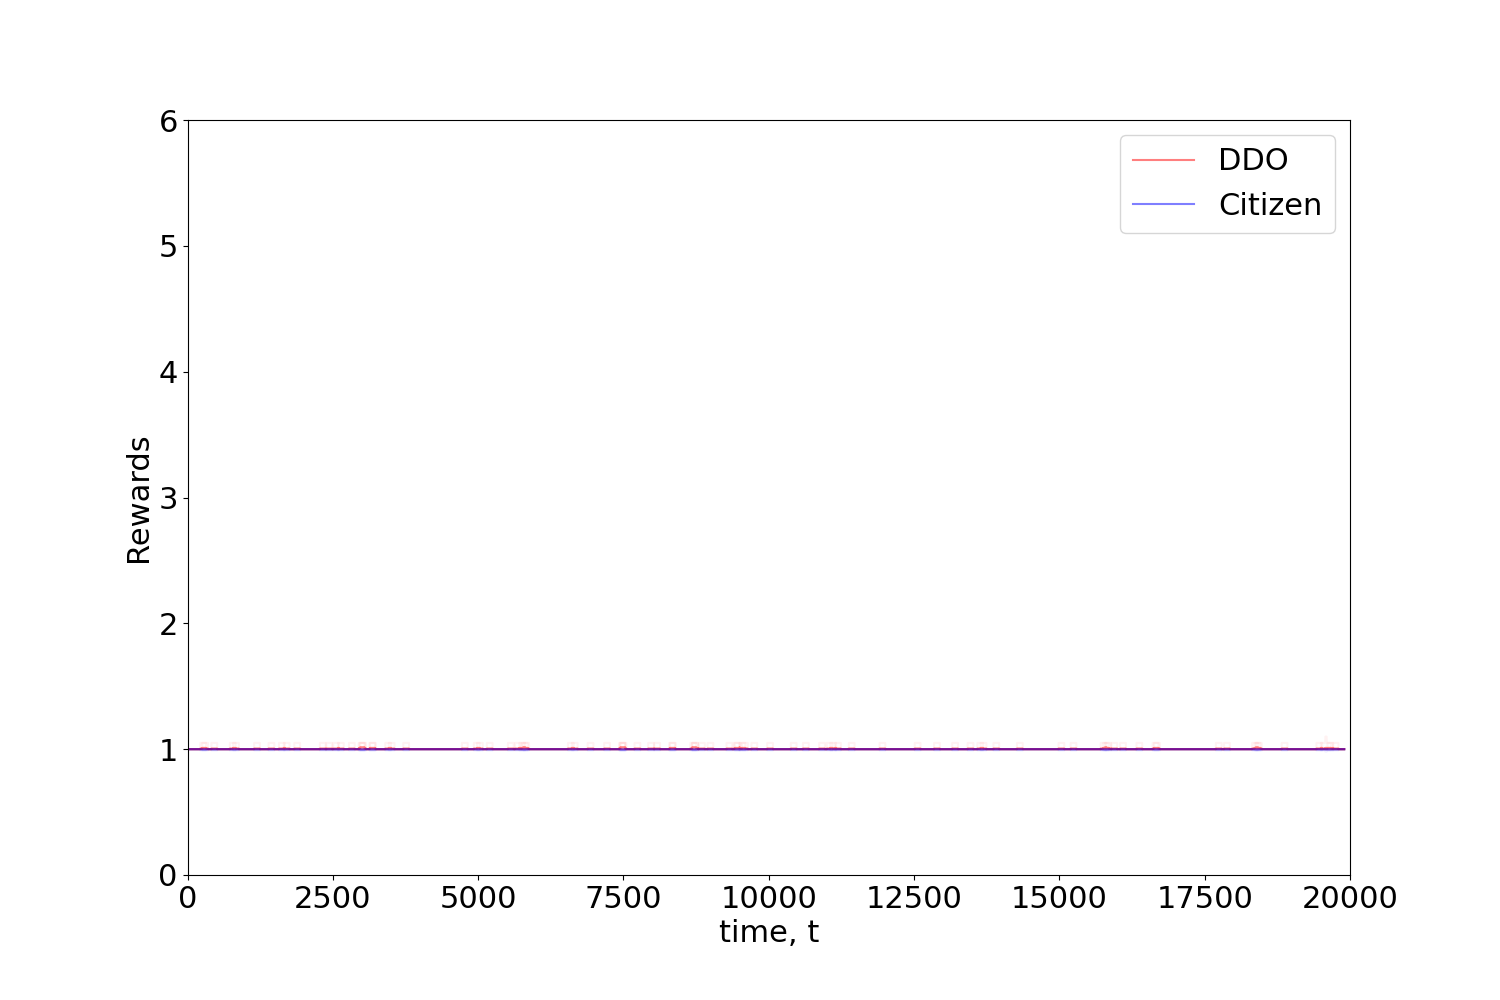
\includegraphics[height=1.8in]{img/selfish_ddo.png}}%
  \subfigure[Social utility.]{%
  \label{fig:nash_sut}%
  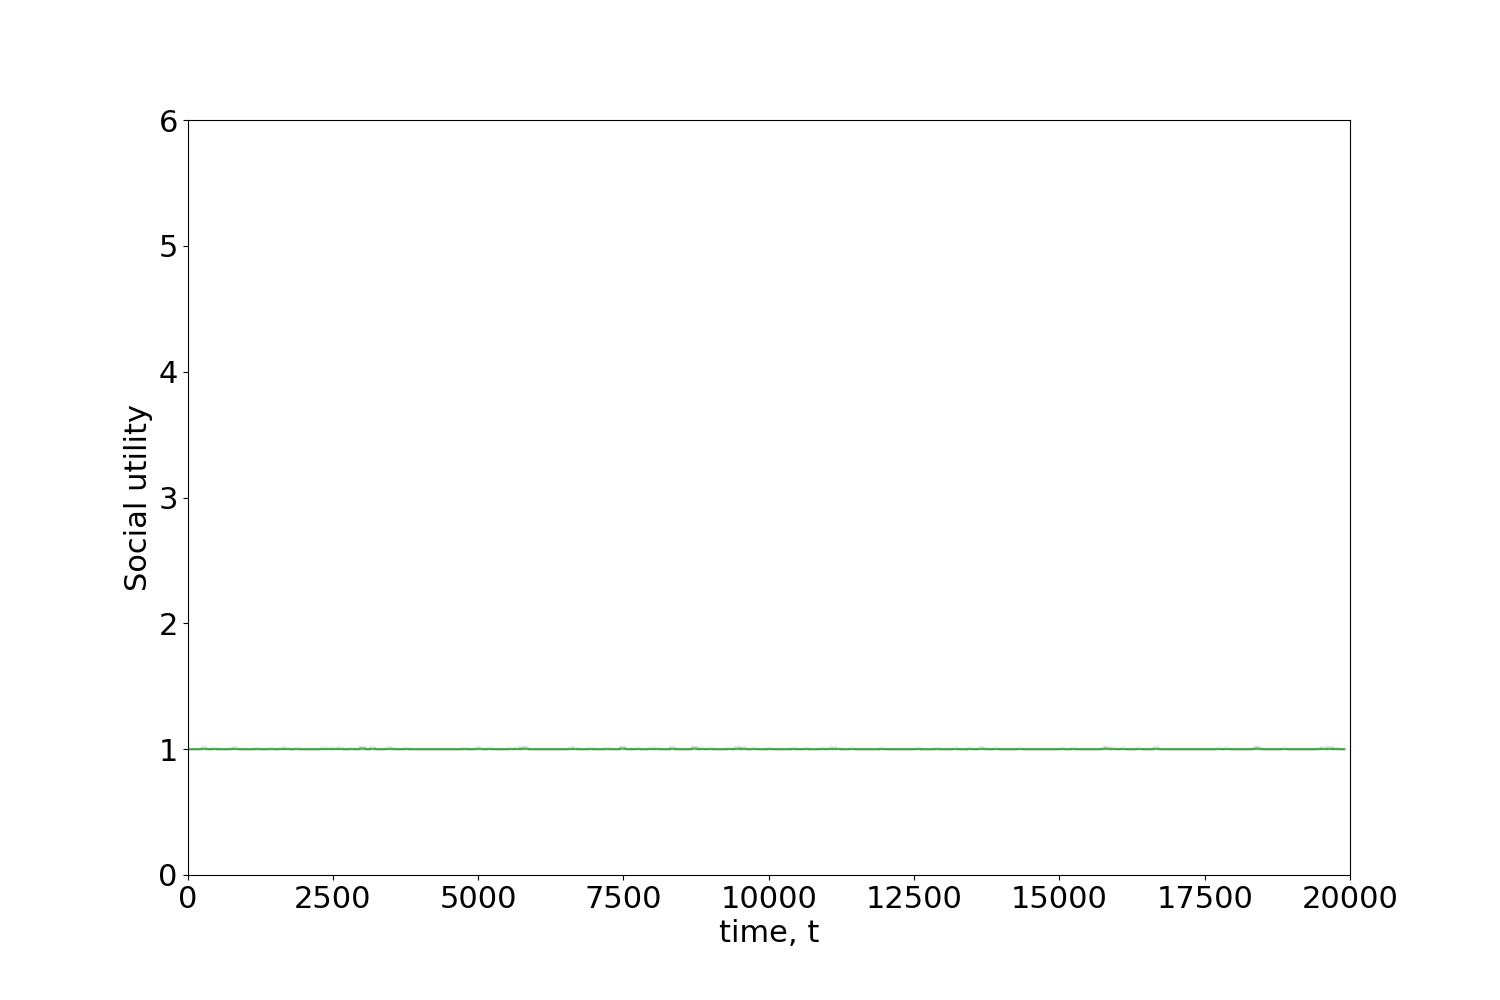
\includegraphics[height=1.8in]{img/selfish_ddo_sut.png}}%
  \caption{Agents' utilities and social utilities in case of DDO always defecting.}
\end{figure*}

\noindent Figure \ref{fig:nash_sut} shows that under the defecting strategy,
the social utility achieves its minimum value. 

%%%%%%%%%%%%%%%%%%%%%%%%%%%
\paragraph{A Tit for Tat DDO}
We next model the DDO as a player using the Tit for Tat (TfT) strategy
(it will first cooperate and, then, subsequently replicate the opponent's previous action: if the opponent was previously cooperative, the agent is cooperative; if not, it defects).
This policy has been widely used in the IPD, because of its simplicity and effectiveness \cite{axelrod84}. A recent experimental study 
\cite{dal2019strategy}
 tested real-life people's behaviour in IPD scenarios,
 showing that TfT was one of the most widely strategies.
 Figure \ref{fig:FPMvsTfT} shows that under TfT, the 
 social utility achieves its maximum value: mutual cooperation is achieved, thus leading to the optimal social utility.

\begin{figure}[h!]
\centering
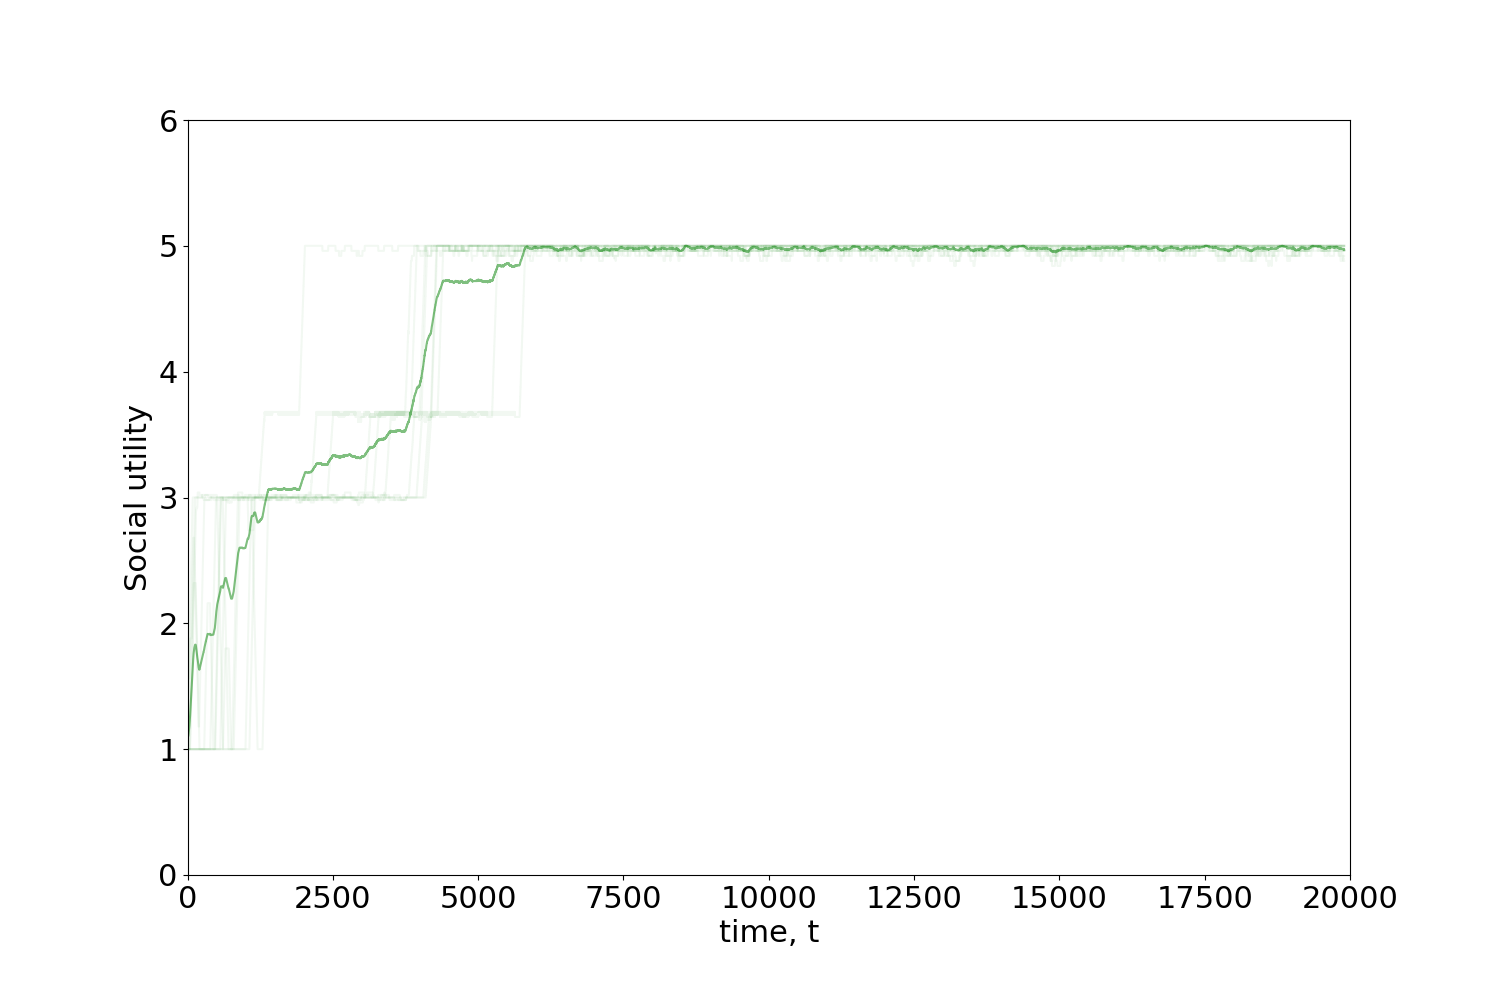
\includegraphics[width=0.6\linewidth]{img/tft.png}%
\caption{Social utility of a FPM citizen against a TfT DDO.}\label{fig:FPMvsTfT}
\end{figure}

\noindent It is important to mention though that 
if the citizen had no memory about previous actions, the policy of the DDO could not be learnt and mutual cooperation would not be achieved.

%%%%%%%%%%%%%%%%%%%%%%%%%%
\paragraph{Random behaviour among citizens}
 Previously,  all citizens were assumed to
 act according to the FPM model.
 However, 
 it is unrealistic to assume
 that the whole population will behave following such complex strategies. A more reasonable
 assumption is to consider having a  subpopulation of citizens that acts randomly. To simulate this, we modify the FP/FPM model drawing a random action with probability $0 < \epsilon < 1$ at each turn. As Figure \ref{fig:25} shows, where we set $\epsilon = 0.7$, this entails an important decrease in social utility. 
%For example, we set $\epsilon = 0.05$ and compete against the TfT DDO, leading to trajectories as in Figure \ref{fig:random}. 
%Observe that even for a small amount of deviation from the FP strategy, the decrease in social utility may be even halved when compared to the previous simulation.

%\begin{figure}[h!]
%\centering
%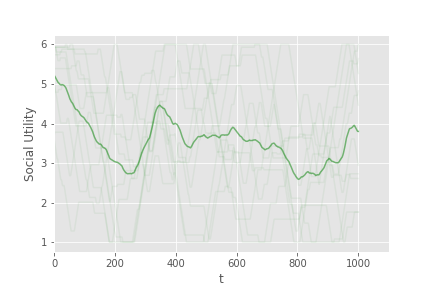
\includegraphics[scale=0.55]{img/random.png}%
%\caption{Social utility when the citizens act randomly %$5$ \% of the time.}\label{fig:random}
%\end{figure}

%%%%%%%%%%%%%%%%%%%%%%%%%%
\paragraph{A forgiving DDO}
A possible solution for this decrease in social utility consists of forcing the DDO to eventually forgive the Citizen and play cooperate, regardless of
her previous actions. We model this as follows: with probability $p$ the DDO will cooperate, whereas with probability $1-p$ he will play TFT. 
%
% \begin{figure*}[h!]
% \centering
% \subfigure[$p=0.25$.]{%
%   \label{fig:25}%
%   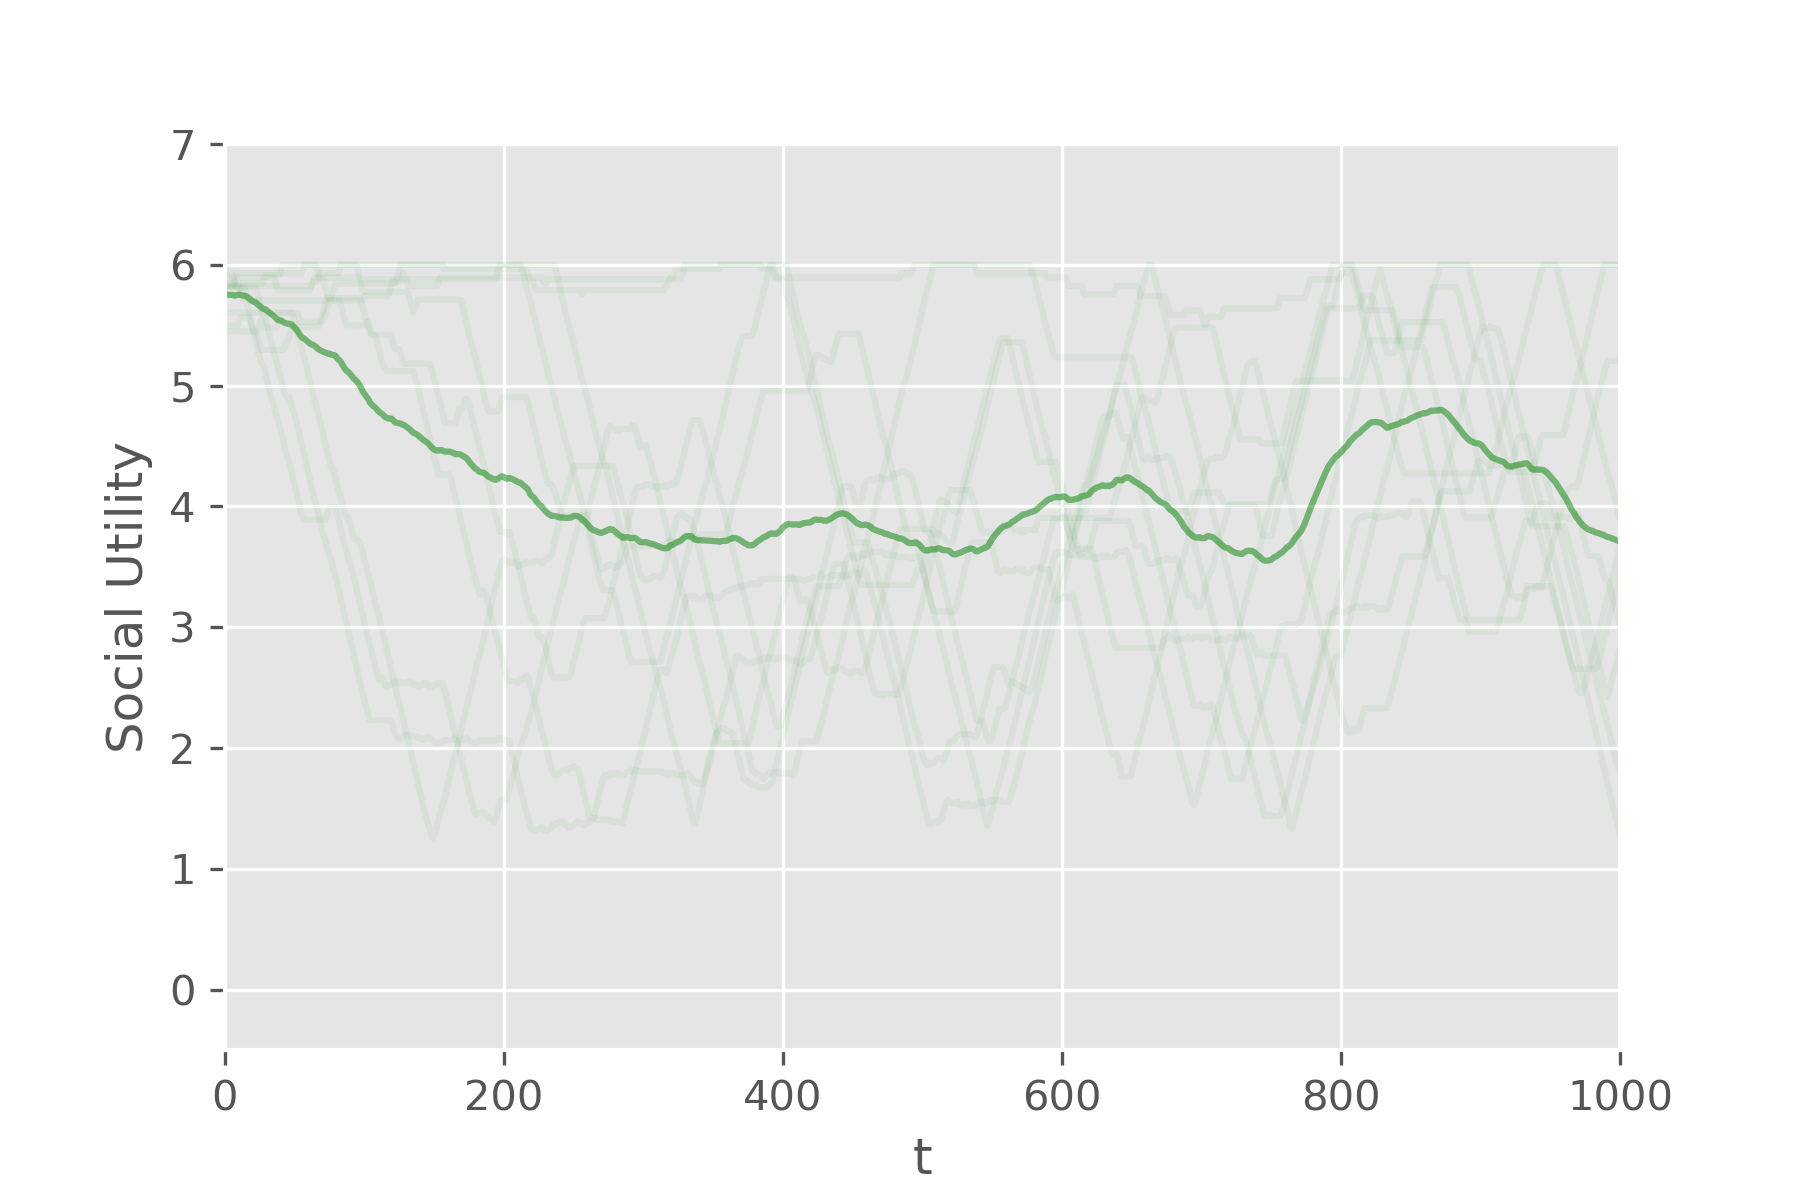
\includegraphics[height=1.8in]{img/SUT_forg1.png}}%
%   \subfigure[$p=0.5$.]{%
%   \label{fig:50}%
%   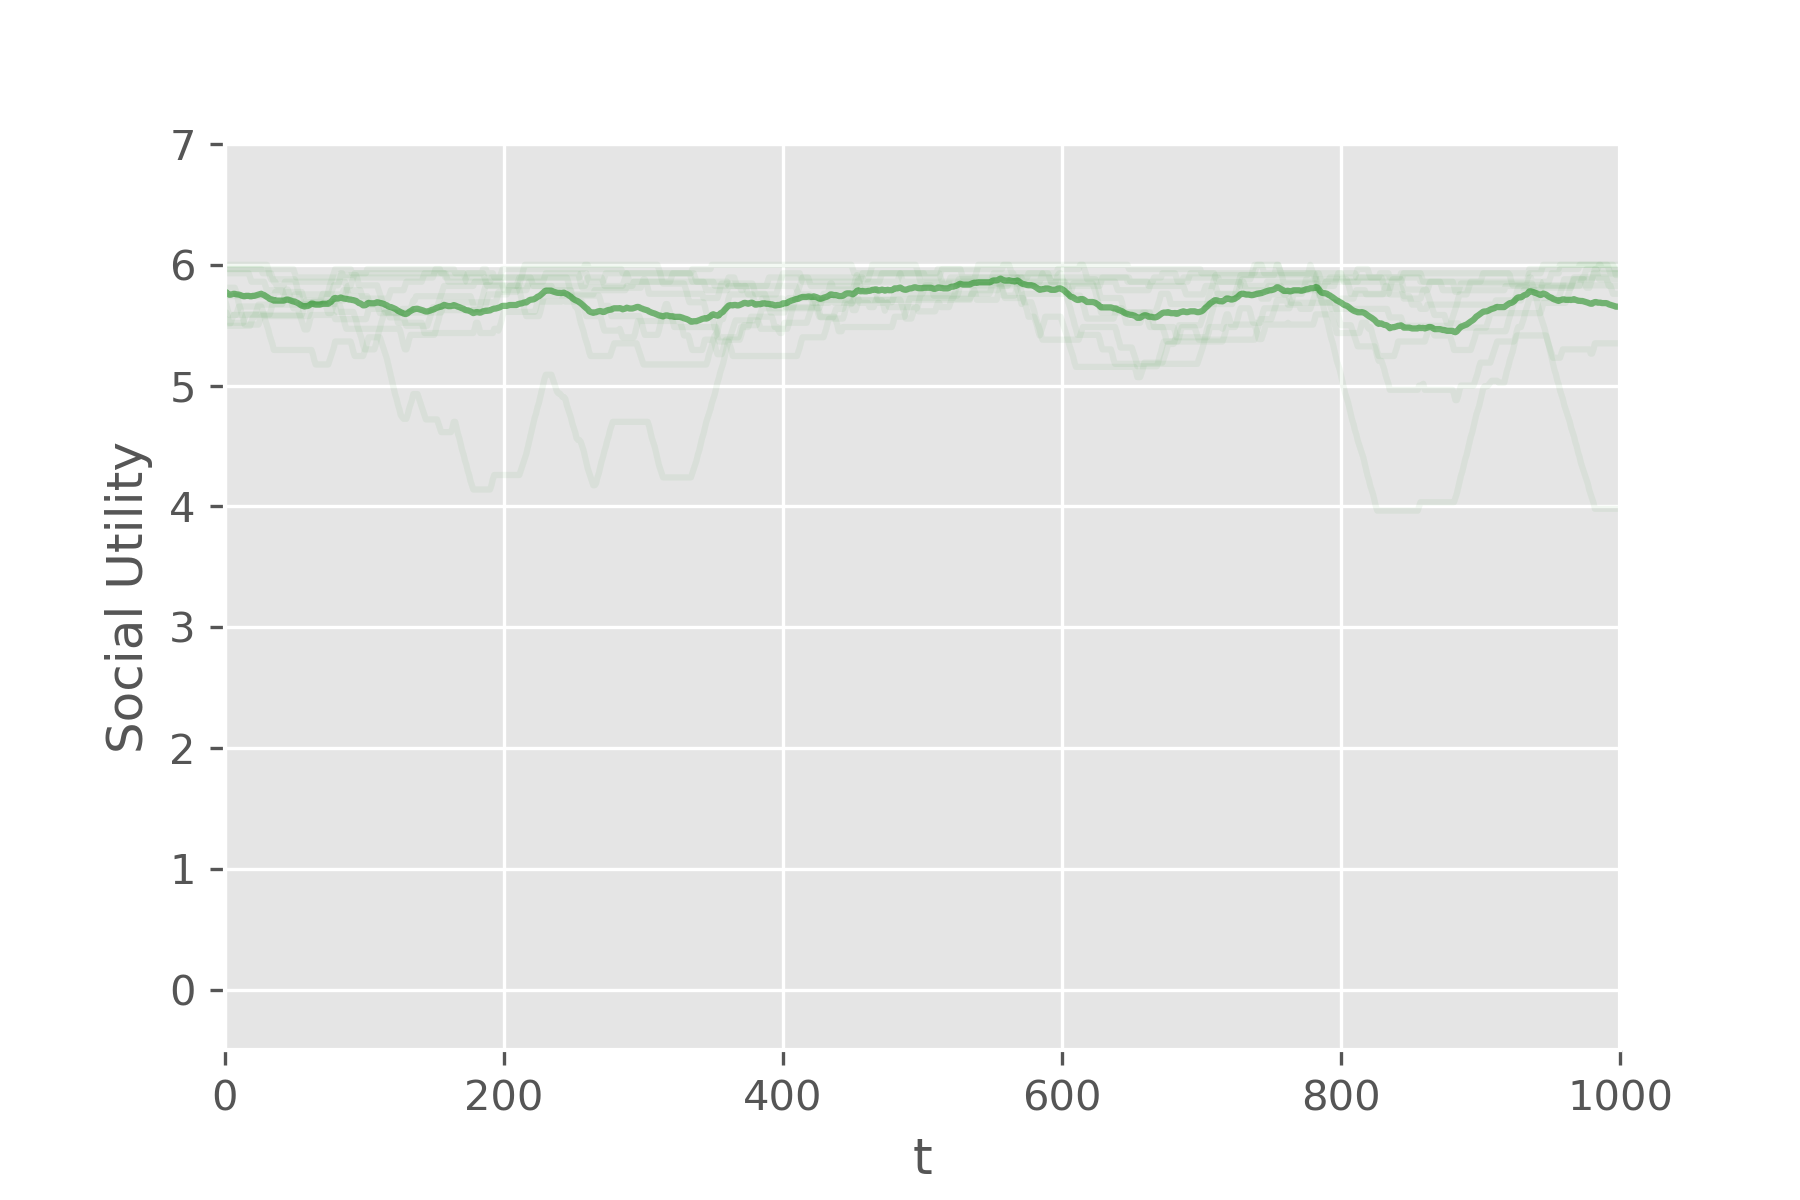
\includegraphics[height=1.8in]{img/SUT_forg2.png}}%
%   \caption{Social utilities for TFT with forgiveness. }
% \end{figure*}
%

\begin{figure}[h!]
\centering
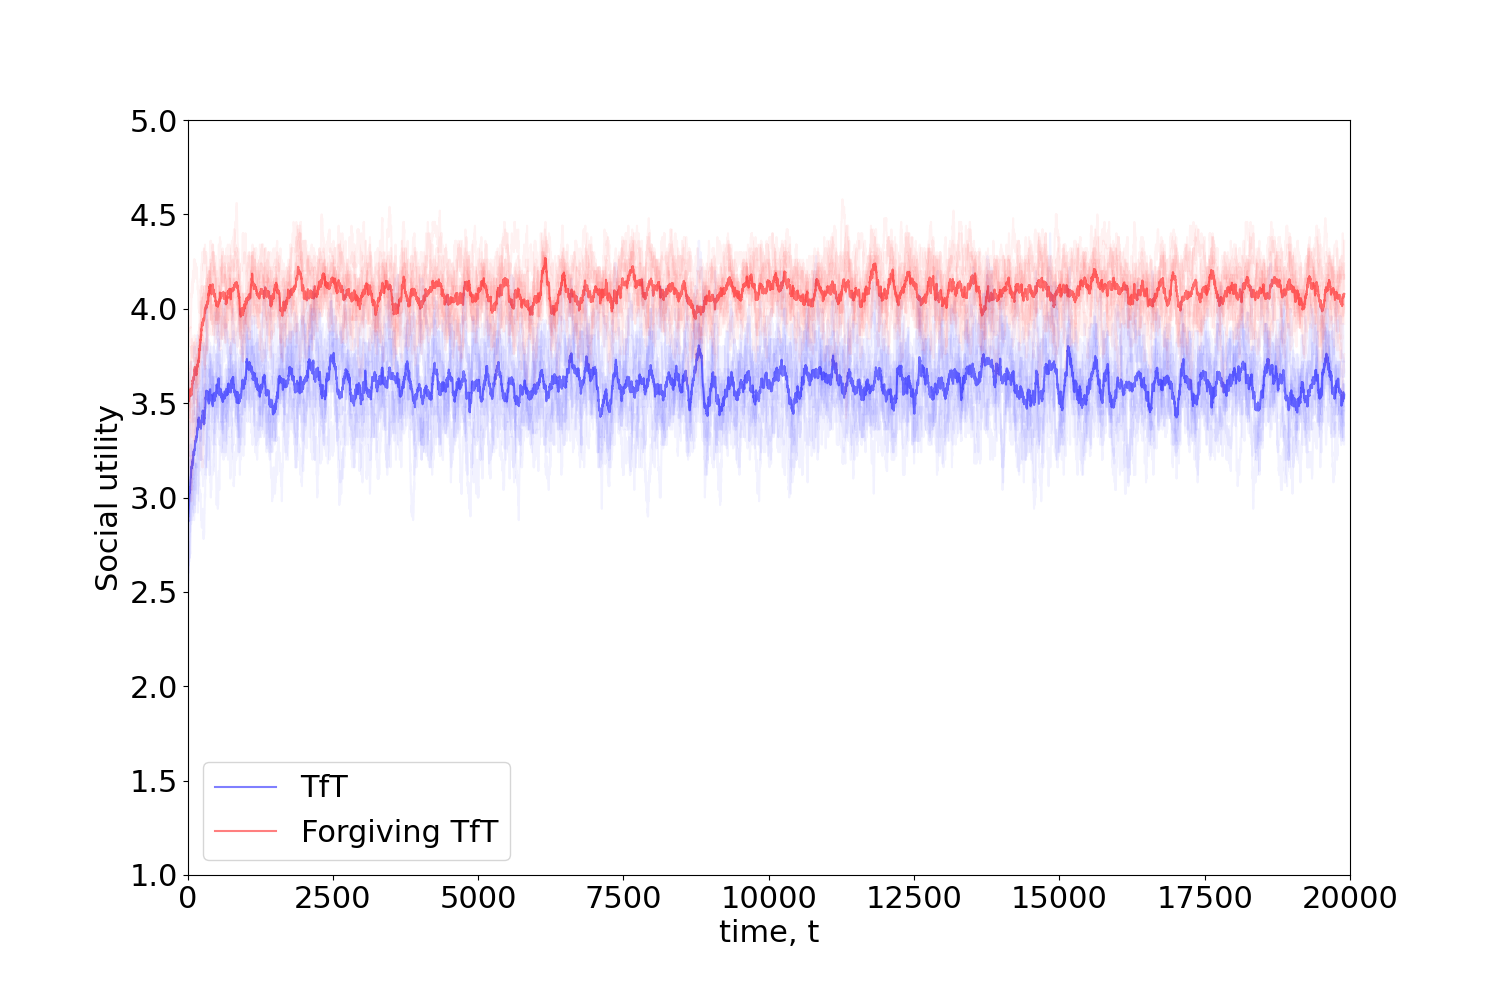
\includegraphics[width=0.6\linewidth]{img/forgiving_tft.png}%
\caption{Social utility when citizens act randomly $70$ \% of the time against a TfT and a forgiving TfT DDO.}\label{fig:25}
\end{figure}

To assess what proportion of time should the DDO forgive, we evaluated a grid of values from 0 to 100, and chose the one that produced the highest increase in social utility. The optimal value was forgiving $70 \%$ of time.
%the same proportion of time that citizens act randomly.
As Figure \ref{fig:25} shows, this produces an increase of approximately half a unit in the average social utility with respect to the case of never forgiving.

Note, though, that there exists a limit value for the forgiving rate such that, if surpassed, the social utility will decrease to around 3. The reason for this is that, in this regime, when not acting randomly, the Citizen will learn that the DDO cooperates most of the time, and thus her  optimal strategy will be to defect. Thus, in most iterations the actions chosen will be $(C, D)$. %, leading to a social utility of around 3.

%Shall the DDO increment his forgiving rate, the social utility won't, as he will tend to play cooperate most of the time, being exploitable by the Citizen.
%Figure \ref{fig:50} shows that forgiving half of the times, makes average social utility to almost reach its maximum value.

%Existe un valor límite (alrededor de 0.8 en este caso), tal que, si superado, la utilidad social baja drásticamente. Esto es así porque, a partir de este valor, el Citizen se da cuenta de que el DDO escoge muy frecuentemente cooperate, entonces él empieza a escoger Defect. Esto hace que la utilidad social baje hasta más o menos 3 ( (6+0)/2 ).


%%%%%%%%%%%%%%%%%%%%%%%%%%%%%%%%%%%
\subsection{Taxation through a regulator}\label{sec:regulator}

Let us discuss an alternative solution to promote cooperation introducing a third player, a Regulator (R, it). Its objective is to nudge the behaviour of the other players through utility transfer, based on taxes.   Appendix \ref{one-shot}
discusses a one-shot version identifying its equilibria.
As in Section 4.1, our focus 
is on the iterated version of this game.

At each turn, the regulator will choose a tax policy for the agents 
$$
(tax_{C, t}, tax_{DDO,t}) \sim \pi_R(\cdot | o_R, \theta_R), 
$$
where $o_R$ is the observed state of the game
and $\theta_R$ are relevant parameters for the regulator. 
Then, the other two agents will receive their corresponding adjusted utility $\tilde{r}_{a,t}$ through 
$$
\tilde{r}_{a,t} = r_{a, t} - tax_{a,t} + \frac{1}{2} \sum_a tax_{a, t},
$$
where the first term is the original utility (Table \ref{tab:payoffIPD});
the second is the tax that the regulator collects 
from that
agent; and, finally, the third one is the (evenly) redistributed collected 
reward.  Note that
$$
SU_t = \frac{r_{C, t} + r_{DDO, t}}{2} = \frac{\tilde{r}_{C, t} + \tilde{r}_{DDO, t}}{2}. 
$$
Thus, under this new reward regime, utility is not created nor destroyed, only transferred between players.

Let us focus now on the issue of how does the Regulator learn its
tax policy. For this, we make it another RL agent that maximizes the social welfare function,
thus optimizing its policy by solving 
$$
\max_{\theta_R} \mathbb{E}_{\pi_R} \left[ \sum_{t=0}^\infty \gamma^t SU_t \right].
$$
Therefore, two nested RL problems are considered: first, 
the regulator selects a tax regime and, next, the other two players optimally adjust their behaviour to this regime. After a few steps, 
the regulator updates its
policy to further encourage cooperation (higher $SU_t$), and so on. At the end of this process, we would expect  both players' behaviours to have been nudged towards cooperation.
 
 We thus frame learning as a bi-level RL problem with two nested loops, 
 using policy gradient methods:
\begin{enumerate}
    \item \textbf{(Outer loop)} The regulator 
    has parameters $\theta_R$, imposing a certain tax policy.
    \begin{enumerate}
        \item \textbf{(Inner loop)} The agents learn under this tax policy for $T$ iterations:
        \item They update their parameters: $\theta_{a, t+1} = \theta_{a, t} + \eta \nabla \mathbb{E}_{\pi_a} \left[ \sum_{t=0}^\infty \gamma^t r_{a, t} \right] $.
    \end{enumerate}
    \item The regulator updates its parameters: $\theta_{R, t+1} = \theta_{R, t} + \eta \nabla \mathbb{E}_{\pi_R} \left[ \sum_{t=0}^\infty \gamma^t SU_t \right]  $.
\end{enumerate}


%TODO: Formalizar un poco convergencia a optimo local


Let us highlight a few benefits of this approach.
First, the regulator makes no assumptions about the policy models of the other players (thus it does not matter whether they are just single-RL agents or are opponent-modelling). Moreover,
the framework is also agnostic to the \emph{social welfare function} to
be optimized; for simplicity, we just use expression (\ref{eq:su}).
%, although one of the
%experiments illustrates the use of a Rawlsian welfare function, focusing on the less privileged agents.  
     It is also scalable to more than two players: 
     the regulator only needs to collect taxes for each player, and then redistribute wealth.
   In presence of $k > 2$ agents, it would have to split the sum of taxes by $1/k$. 
   %  Finally,
%    this framework could also be implementable in real-life settings: R creates a market in which players share information, paying or receiving a certain quantity of money which is dynamically adjusted with the current tax policy.

%%%%%%%%%%%%%%%%%%%%%%%%%%%%%%%%%
\subsubsection{Experiments}

This experiment 
illustrates %the performance of the general 
%framework, showing 
how the inclusion of a Regulator encourages the emergence of cooperative behavior.

Consider the interactions between a Citizen and a DDO. 
The parameter for 
each player is a vector $\theta_a \in \mathbb{R}^2$, with $a \in \lbrace C, DDO\rbrace $, representing the logits of choosing the actions,
i.e. the unnormalized probabilities of choosing each decision.
We consider two types of regulators.

The first one has a discrete action space defined through
 % \[
 %   \begin{array}{lr}
 %       tax_{a,t} = 0.00 & \text{if } a_R = 0\\
 %       tax_{a,t} = 0.15\cdot r_{a,t} & \text{if } a_R = 1\\
 %       tax_{a,t} = 0.30\cdot r_{a,t} & \text{if } a_R = 2\\
 %       tax_{a,t} = 0.50 \cdot r_{a,t} & \text{if } a_R = 3.\\
 %       \end{array}
 % \]
$$
        tax_{a,t} =  \begin{cases} 0.00 & \text{if } a_R = 0\\
        0.15\cdot r_{a,t} & \text{if } a_R = 1\\
        0.30\cdot r_{a,t} & \text{if } a_R = 2\\
        0.50 \cdot r_{a,t} & \text{if } a_R = 3. \end{cases}
$$
For example, when $a_R=2$ the tax rate reaches 30\%.
In this case, $\theta_R \in \mathbb{R}^4$ represent the 
logits of a categorical 
random variable taking the previous values (0,1,2,3).

The second regulator adopts a Gaussian policy defined 
through $\pi_R(d_R | o_R, \theta_R) \sim \mathcal{N}(d_R | \theta_R, 0.05^2)$, with tax 
$$
tax_{a,t} = 0.5 \cdot sigmoid(d_R) \cdot r_{a,t},
$$
to allow 
for a continuous range in $\left[ 0, 0.5 \right]$.

Experiments run for $T=1000$ iterations.
After each iteration, both agents perform one update of
their policy parameter gradient.
The regulator updates its parameters using policy gradients every 50 iterations.
The decision of updating the regulator less frequently than the other agents is motivated to allow them to learn and adapt to the new tax regime and stabilise
 overall learning of the system.
Figure \ref{fig:su} displays results. 
 For each of the three variants (no intervention, discrete, continuous) we plot 5 different runs and their means in darker color.
 
\begin{figure}[!h]
\centering
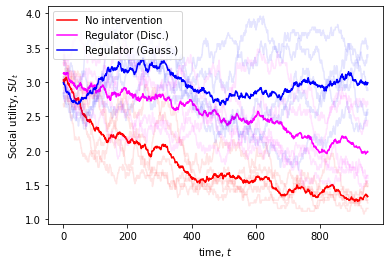
\includegraphics[width=0.55\linewidth]{img/su.png}
\caption{Social utility under three different regulation scenarios.}\label{fig:su}
\end{figure}

 Clearly, under no intervention, both agents fail to learn to cooperate
converging to the static 
Nash equilibrium $(D,D)$. 
We also appreciate that the discrete policy is neither 
effective, also converging to $(D,D)$, albeit at a much slower pace.
On the other hand, the Gaussian regulator is 
 more efficient as it allows to avoid convergence to $(D,D)$
although it does not preclude convergence to $(C,C)$.
This regulator is more effective than its discrete counterpart,
because it can better exploit 
the policy gradient information. Because of this, 
in the next subsection we focus on this Gaussian regulator.

In summary, the addition of a Regulator can make a positive impact in the social utility attained in the market, preventing collapse into $(D, D)$. However, introducing taxes is not sufficient, since in Figure \ref{fig:su} the social utility converged towards a value of 3, far away from the optimal value of 5.
%%%%%%%%%%%%%%%%%%%%%%%%%%%%%%%%%%%%%%%%%%%%%
\iffalse
\paragraph{An egalitarian society} 
Next, instead of the social utility (\ref{eq:su}),
we consider a Rawlsian utility function defined at each timestep $t$ through
$$
RU_t = \min \lbrace r_{C,t}, r_{DDO, t} \rbrace.
$$
The rest of the setup is as before.
Results are shown in Figure \ref{fig:ru}.


\begin{figure}[!h]
\centering
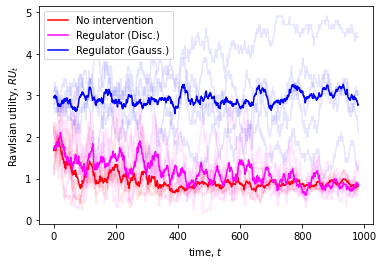
\includegraphics[width=0.6\linewidth]{img/ru.png}
\caption{Rawlsian utility under three different scenarios.}\label{fig:ru}
\end{figure}
 \noindent As before, the introduced Regulator framework improves cooperation, even under a different utility function. This highlights another of main the benefits of the Regulator framework: it can nudge the behaviour of the agents towards
 optimizing any desired social welfare function, while being agnostic to the underlying behavior model of the participating agents.
\fi

%subsection{Further work}


%begin{itemize}
%item Introduce ideas from metalearning/VIS to adapt the learning rate of the Regulator, to further improve convergence of the others.
%item More complex tax schema?
%item More players?
%end{itemize}


\subsection{Introducing incentives}\label{sec:incentives}


In order to further stimulate cooperative behavior, we introduce incentives to the players via the Regulator: if both players cooperate at a given turn, they will receive an extra amount $I$ of utility,
 a scalar that adds to their perceived rewards. Appendix  \ref{sec:oneshot_inc} shows that incentives complement well with the tax framework, so that mutual cooperation is possible in the one-shot version of this game. Note that, when $I>T-R$, instead of the Prisoner's Dilemma, we have an instance of the Stag Hunt game \cite{skyrms2004stag}, in which both $(C, C)$ and $(D, D)$ are 
 pure Nash equilibria.\footnote{Achieving mutual cooperation is much simpler in this case.}

As before, we focus the discussion in the iterated version.
%This new mechanism is straightforward to implement: if both players cooperate at any given turn, the Regulator adds the same incentive to both players. This incentive  is a scalar that adds to their perceived rewards.
In this batch of experiments, players interact over $T=1000$ iterations, and the Regulator only provides incentives during the first 500 iterations. After that, it will only collect taxes from the players and redistribute them as in Section \ref{sec:regulator}. Figure \ref{fig:inc1} shows
results from 
several runs under different incentive values. A few comments are in order.

\begin{figure}[!h]
\centering
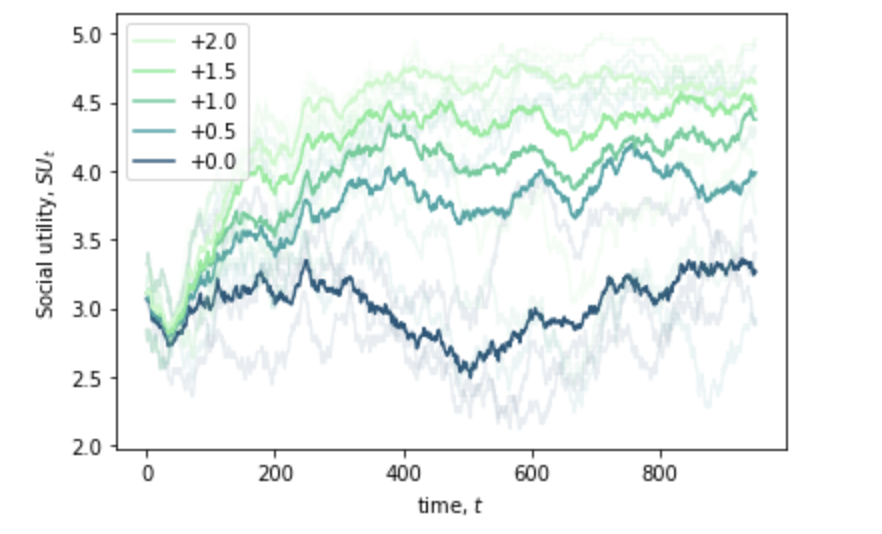
\includegraphics[width=0.6\linewidth]{img/inc1.png}
\caption{Social utility under different incentives with tax collection.}\label{fig:inc1}
\end{figure}

\begin{figure}[!h]
\centering
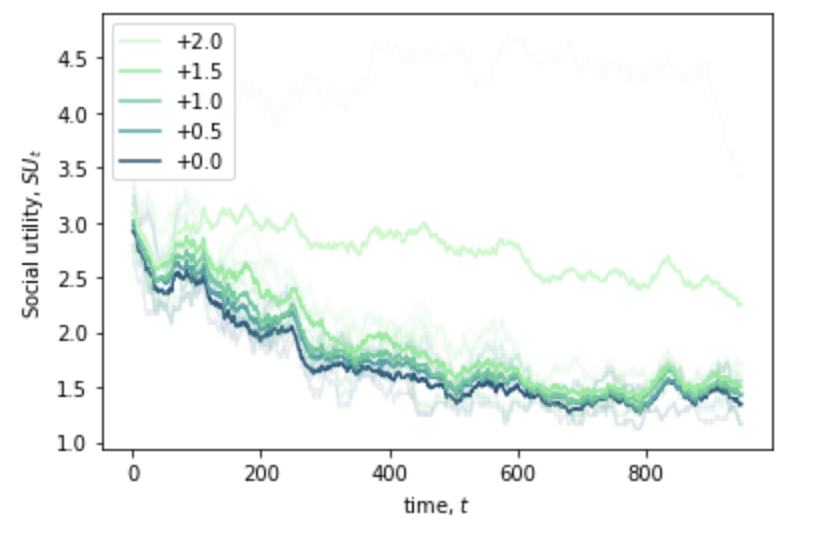
\includegraphics[width=0.6\linewidth]{img/inc2.png}
\caption{Social utility under different incentives with no tax collection.}\label{fig:inc2}
\end{figure}


Firstly, note that as the incentive increases, also does the social utility.
For an incentive of 1, the maximum reward of $(C, C)$ and $(D, C)$ is the same (6) for the Citizen, and cooperation naturally emerges. Also note that since the policies for each player are stochastic, it is virtually impossible to maintain an exact convergence towards the optimal value of 5, since a small amount of time the agents are deviating from $(C,C)$ due to the stochasticity in their actions. Second,
observe that even when the Regulator stops incentives to players in the middle of the simulations, both players keep cooperating along time.

We hypothesize that the underlying tax system from Section \ref{sec:regulator} is necessary for players to learn to cooperate and maintain that behaviour even after the Regulator ends up incentives. To test this hypothesis, we repeat the experiments removing tax collection, \emph{ceteris paribus}. Results are shown in Figure \ref{fig:inc2}. Observe now that even under the presence of high incentives, both agents fail to cooperate, with social utility decaying over time. Thus,  the tax collection framework from \ref{sec:regulator} has a synergic effect with the incentives introduced in this Section.




